\chapter{4. Small Scale Prototype}

As a first step towards the design and fabrication of a tilting PEV, an small scale prototype was built. In this chapter the design and fabrication process regarding this small vehicle, also called \textbf{miniPEV}, will be explained.

\section{Concept - Deploy or Die}

In sight of the Media Lab's motto '\textbf{deploy or die}'\cite{deploydie}, the objective of this thesis would be to deploy a real scale vehicle with a tilting mechanism. However, the process to reach that goal needs a lot of iterations, try and errors, and a small scale prototype is a good starting point.

\begin{marginfigure}
	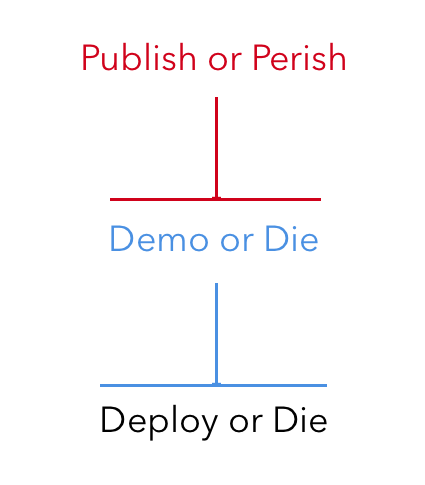
\includegraphics[width=1.1\linewidth]{figs/04/deploy_die}
	\caption{Evolution of the philosophy of innovation at the Media Lab}
\end{marginfigure}

A small moving tilting prototype  -- \textbf{miniPEV}-- is helpful in a lot of different ways. It is much easier to show your ideas and the story behind narrow tilting vehicles to people who are not familiarized  with this kind of vehicles. As a matter of fact, the miniPEV was shown in the Fall Member Event at the Media Lab. The feedback received from the sponsors, students, and people from the MIT community was really helpful to understand better the problem and its opportunities in the mobility sector.

The miniPEV\cite{miniPEV} is a simple tilting 'toy' car make out of wood. It is approximately one quarter of the scale of the PEV, but as a concept, it represents all the features that a full scale vehicle has.
It is propulsed by a DC motor, and two servomotors move the two front steering wheels and the tilting mechanism. It also has a battery to power all the electronics and the motors. In order to simulate the same inputs to the control system, a Inertial Measurement Unit (IMU) was also installed and used to tilt the vehicle in the curves. The details regarding the components will be explained later in this chapter.



\newpage
\section{Design}

The design on the miniPEV was based on a previous small prototype by Michael Lin, head of the PEV project at Changing Places group. In order to fabricate the prototype as fast as possible, the miniPEV was built with plywood sheets of $3mm$, that were cut in the laser cutting machine. Then, gluing the layers together gives result to the final 3D model. In this way, the prototype is fabricated very fast and the possibilities of making changes is high as well.

The model is composed of different parts. In the rear part there is a seat, and the wheel is propulsed from the hub. The electronics and the battery are placed in the center, with the aim of keeping the model as balanced as possible and having a low center of gravity. Due to the limitations of power, this design decision was critical for the proper motion of the model. The front part consist of two steered wheels with their steering system and a suspension that allows the tilting of the vehicle.

\section{Tilting Mechanisms}

This section focuses on explaining the tilting mechanism chosen for the miniPEV, as an introduction to the more detailed simulations carried out for the full scale PEV. 

The different tilting mechanisms that previous tilting vehicles have used can be summarized in two categories:
\begin{enumerate}
\item \textbf{Hydraulic actuators}: located in the suspension or in a fixed part of the vehicle, they can incline the vehicle by extending one of the two actuators. The size and power provided by these actuators exceed the requirements and the space available in the PEV, as well as in the miniPEV. This strategy has been used in car-like vehicles rather than in bike-like vehicles.

\item \textbf{Rotary motor}: being much compact, a high torque motor can supply the necessary $M_{t}$ to lean the vehicle when necessary. Here the possibilities of actuating the vehicle expand, but the design remains basic. Attached to the motor there is a arm that connects to the suspension arms, meaning that the rotation of the motor reduces and enlargers the distance from the body to the suspension, hence tilting the vehicle and the wheels. This second option is the one that is going to be explored next, due to the different possibilities that comprises.
\end{enumerate}

\newpage
\textbf{Rotary Motor Tilting Mechanisms}

If a rotary motor is used, the first question that arises is: What part of the vehicle would we like to tilt? The answer falls on selecting the parts that we do not want to lean. In a tadpole vehicle like PEV with 2 front wheels and 1 rear wheel (the contrary will be a delta vehicle - 1F2R), the part that can maintain vertical by itself is the front suspension and the wheels. In this way, we could separate the whole front part from the rest of the frame (handle bar, cover, seat, rear wheel...), implying that the tilting part would be the body of the vehicle. This is indeed the alternative \textbf{A} (Figure \ref{design_tilting}):

\begin{figure}[h!]
	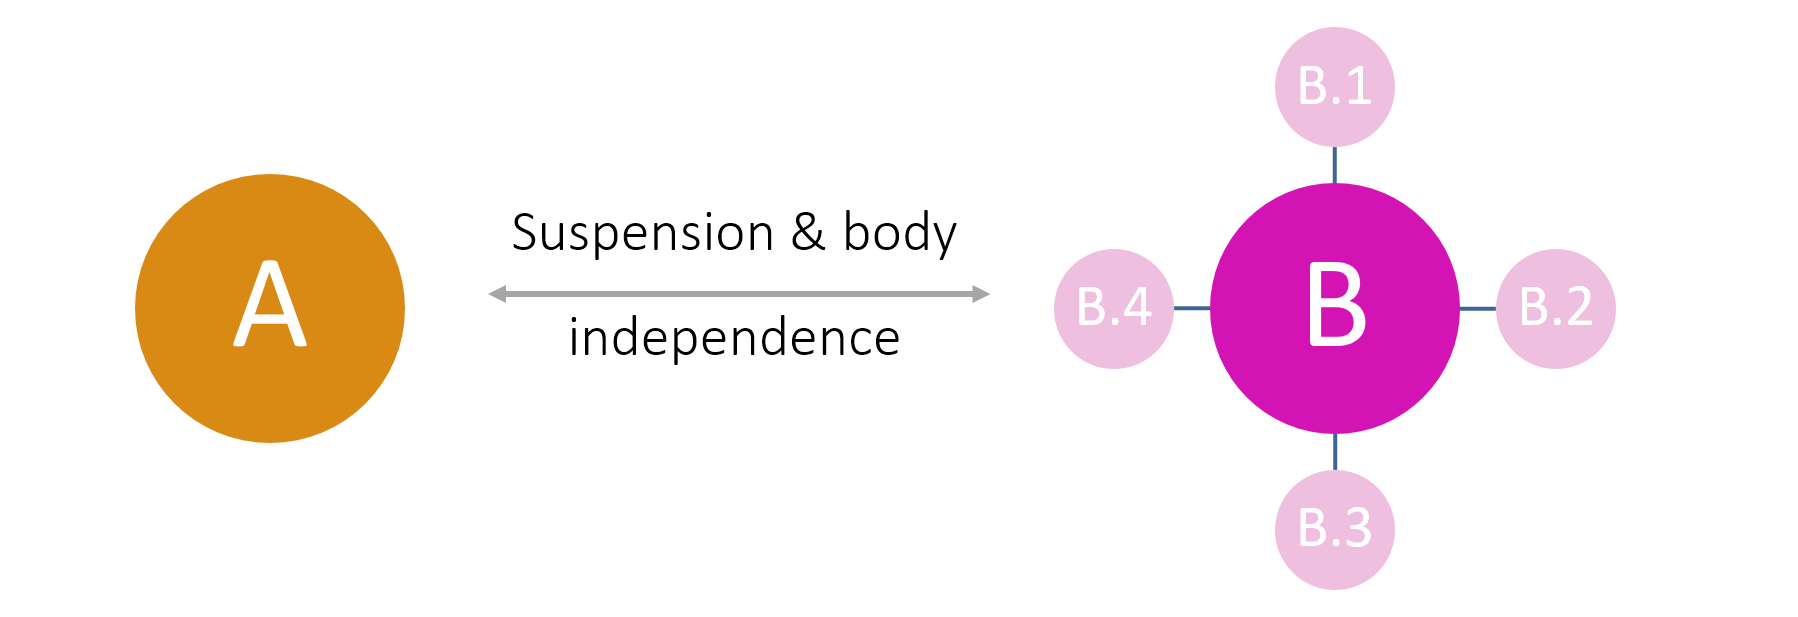
\includegraphics[width=1.0\linewidth]{figs/04/Picture2}
	\caption{Tilting mechanisms alternatives based on the suspension and body independence}
	\label{design_tilting}
\end{figure}

\textcolor{Bittersweet}{A: Separate body from suspension}

In this case the front suspension does not lean, it maintains as if the vehicle did not have a tilting degree of freedom and the wheels maintain vertical as well. Therefore, the suspension keeps its design objective: to absorb the vibration and the bumps reactions coming from the irregular profile of the ground. The current design of the suspension could be used for this tilting PEV. 

On the other side, the junction part between the two parts supposes a high risk point, since all the forces in the vehicle will be concentrated in that point. In addition, it would require to re-design the steering mechanism, since there is a mismatch between the two parts.
\begin{marginfigure}
	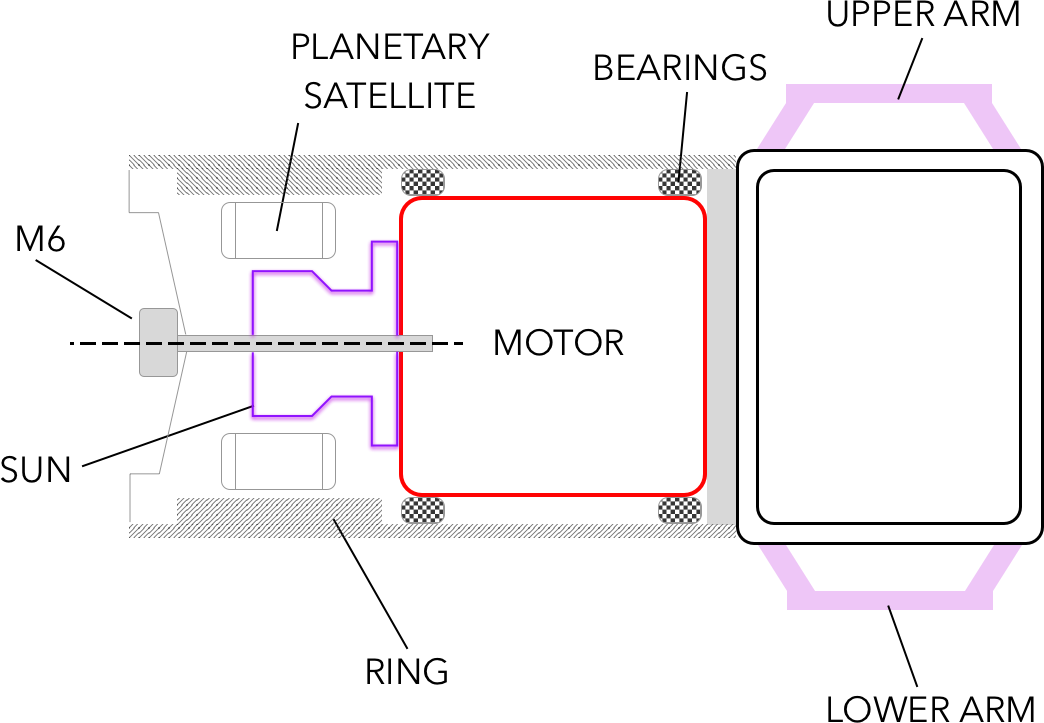
\includegraphics[width=1.2\linewidth]{figs/04/a_option}
	\caption{Design proposal in the joint with option A}
\end{marginfigure}
\begin{itemize}
\begin{itemize}\itemsep -10pt
    \item[$\textcolor{Green}{\surd}$] Suspension does not lean, wheels maintain vertical
    \item[$\textcolor{Green}{\surd}$] Suspension used for vibration absorption
    \item[$\textcolor{Green}{\surd}$] No changes in suspension design
\end{itemize}
\end{itemize}

\begin{itemize}
\begin{itemize}\itemsep -10pt
    \item[$\textcolor{Red}{\times}$] Robust design required, risk point
    \item[$\textcolor{Red}{\times}$] Concentration of forces in the joint
    \item[$\textcolor{Red}{\times}$] Steering re-design
\end{itemize}
\end{itemize}

\newpage
\textcolor{RubineRed}{B: Body moves with suspension}

When the vehicle leans with the suspension, then the wheels also tilt (the camber changes) and there is no risk point since all the frame parts are joint together. Apart from small changes, the steering system can be maintained, which is a advantage. However, this alternative also gives rise to other issues. Leaning the wheels can imply an instability in the vehicle, since some tires are not designed to be tilted an elevate angle. There are also a great deal of actuation strategies, which can be difficult to choose from. 

Nevertheless, the main drawback of this design is that the suspension is not anymore independent from the leaning on the vehicle. This implies that the suspension shock absorbers need to change their position and that the motor actuation cannot conflict with the motion of the suspension due to vibrations or bumps. This issue is really challenging, and in this project we were not able to design a front suspension that separated the suspension motion from the tilting motion. We will sacrifice the absence of the suspension for the sake of reaching to a new concept of tilted tricycle.
\begin{itemize}
\begin{itemize}\itemsep -10pt
    \item[$\textcolor{Green}{\surd}$] Suspension and wheels do lean
    \item[$\textcolor{Green}{\surd}$] Robust design: no risk point
    \item[$\textcolor{Green}{\surd}$] Keep steering design
\end{itemize}
\end{itemize}

\begin{itemize}
\begin{itemize}\itemsep -10pt
    \item[$\textcolor{Red}{\times}$] Suspension not independent from leaning
    \item[$\textcolor{Red}{\times}$] Multiple actuation strategies
    \item[$\textcolor{Red}{\times}$] Stability of the wheels
\end{itemize}
\end{itemize}

To understand the different tilting suspensions, the program Autodesk ForceEffect software was used as a first approach. The suspension was modelled in a 2D plane, with only 1 degree of freedom (which accounts for the leaning of the suspension). 

\begin{figure}[h!]
	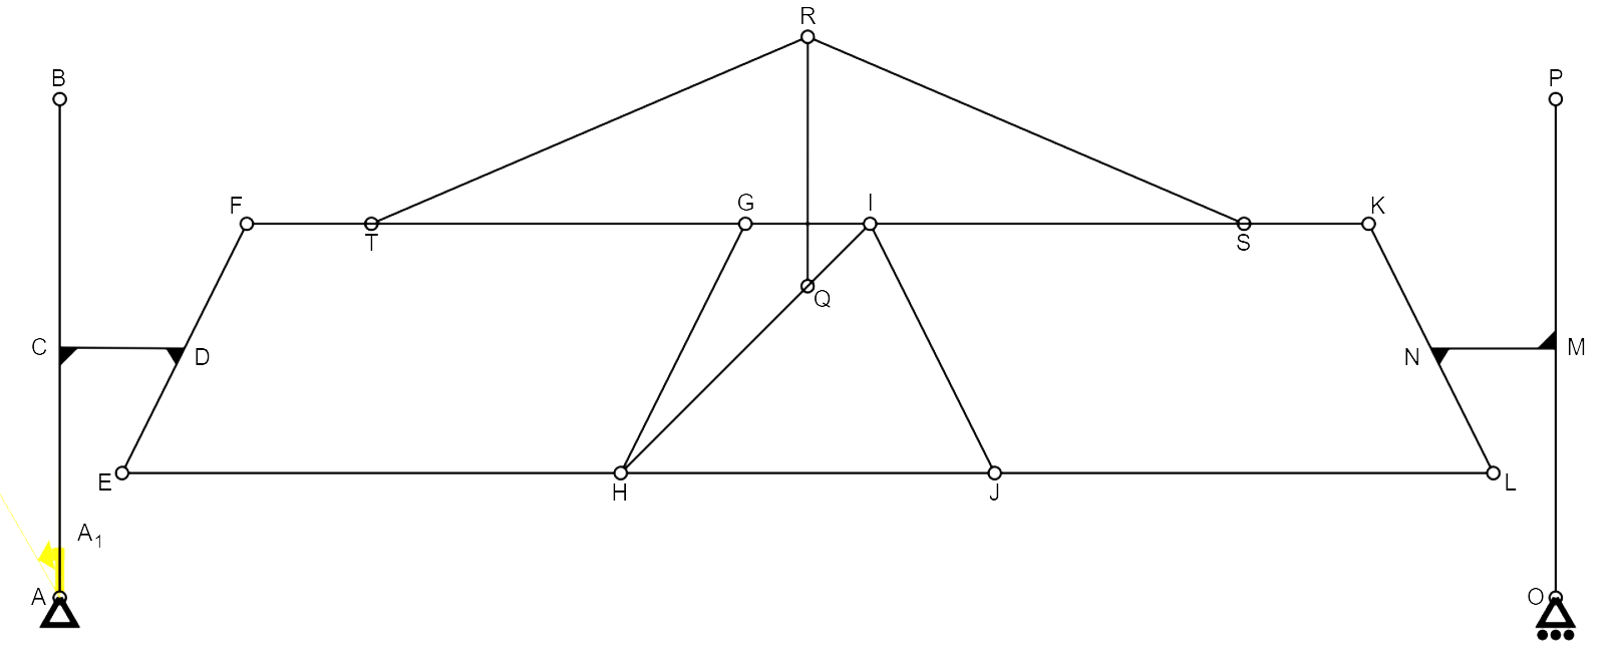
\includegraphics[width=1.0\linewidth]{figs/04/b}
	\caption{Front suspension model in 2D}
\end{figure}

\newpage
The main parts and the links between them are, from left to right:

\begin{itemize}
\begin{itemize}\itemsep -10pt
	\item \textit{Wheel (Left)}: Co-linear bars $\overline{AC}$ and $\overline{BC}$. Point A is in contact with the ground by an articulation. Distance $\overline{AC}$ represents the radius of the front wheel.
	\item \textit{Kingpin (Left)}: Co-linear bars $\overline{DE}$ and $\overline{DF}$. It is inclined by the kingpin angle. 
	\item \textit{Hub (Left)}: $\overline{CD}$ bar, welded to the left wheel and the kingpin.
	\item \textit{Upper/Lower Suspension Arms}: bar $\overline{FG}$/$\overline{EH}$ articulated in both sides.
	\item \textit{Body}: it represents the frame of the vehicle, where the driver will be sitting. Four-sided solid body $GHIJ$.
	\item \textit{Rotation Point}: $Q$ is the point from which the motor will actuate.
	\item \textit{Tilting Mechanism}: Bars $\overline{QR}$ and $\overline{RT}$/$\overline{RS}$.
	\item \textit{Wheel (Right)}: Co-linear bars $\overline{QO}$ and $\overline{OR}$. Point Q is in contact with the ground by a slider.
\end{itemize}
\end{itemize}

With this basic model in mind, the four studied alternatives can be summarized as follows. A more detailed analysis of the front suspension will be explained in the next chapter as well.

\begin{itemize}
\begin{itemize}
	\item \textbf{B.1 Rotating point on top of body + linkage (shock absorbers) to upper arms}
	
	\begin{figure*}[h!]
		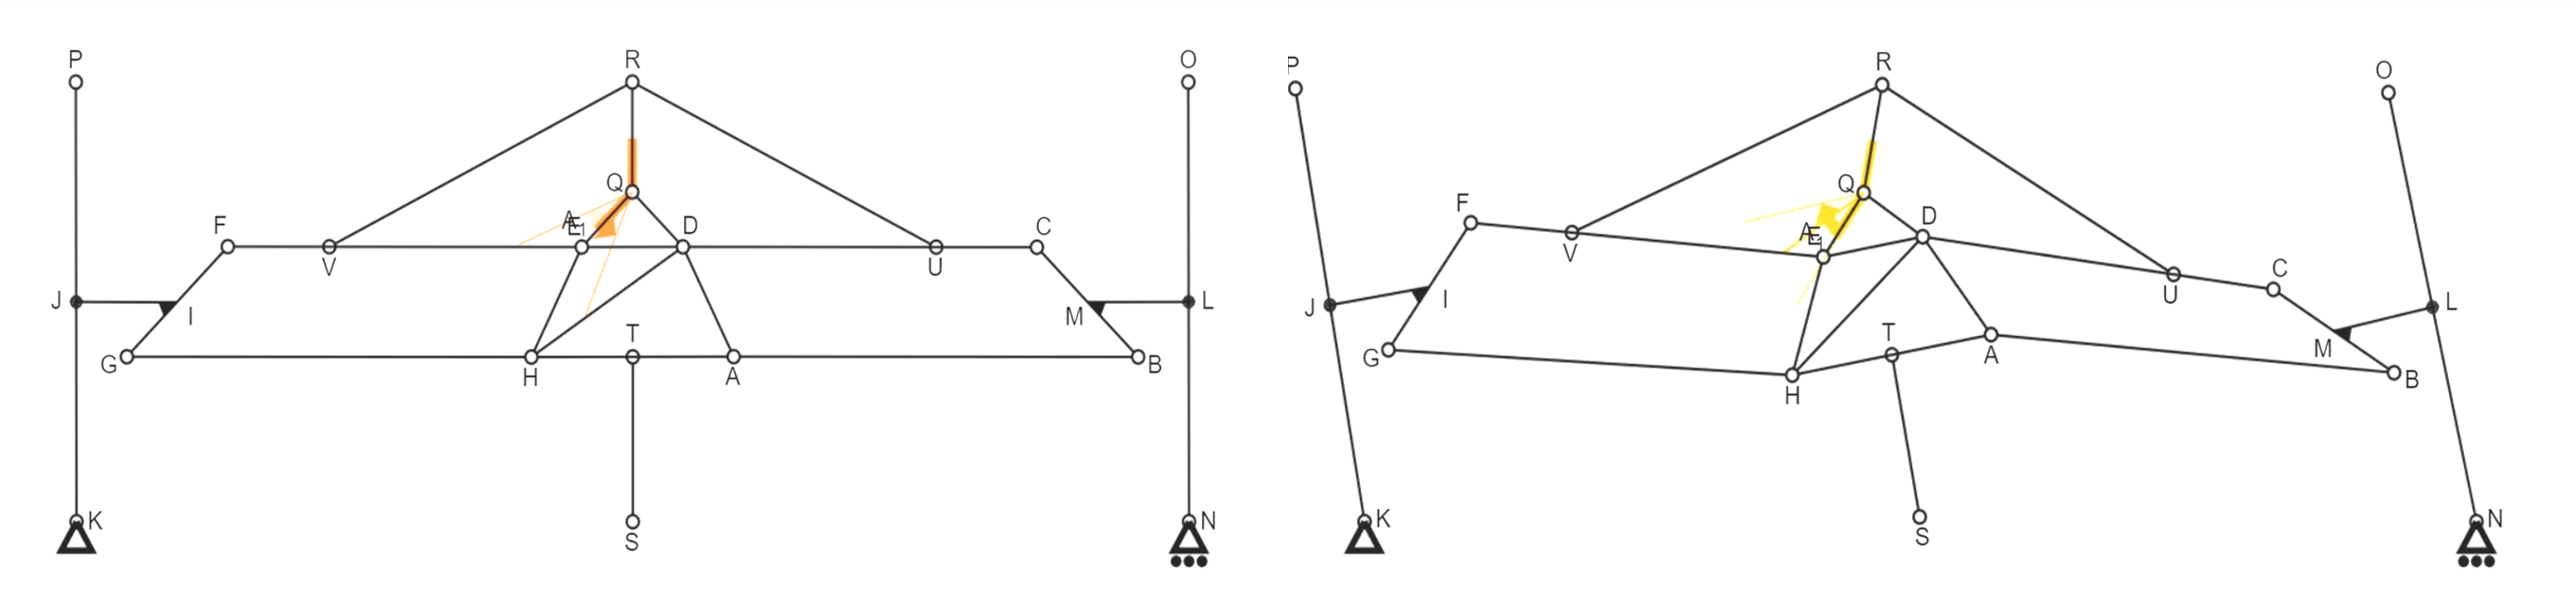
\includegraphics[width=1.1\linewidth]{figs/04/b_1}
		\caption{$B_{1}$ option}
	\end{figure*}
	The tilting mechanism consists of three elements. The arm $\overline{QR}$ is actuated by the motor, and the two remaining bars ($\overline{RU}$ and $\overline{RV}$) are connected to the upper arms. This is the bar system used in the miniPEV. It is a very simple mechanism, but in terms of geometry, requires an angle of \textbf{45 degrees} between the $\overline{QR}$ and $\overline{RU}$ bars in order to get maximum torque on the suspension bars. The rotation point $Q$ is constrained to be on top of the body, and considering the length of the $\overline{QR}$ bar, the space requirement is high.
	\newpage
	\item \textbf{B.2 Rotating point below body + linkage (shock absorbers) to lower arms}
	
	\begin{figure*}[h!]
		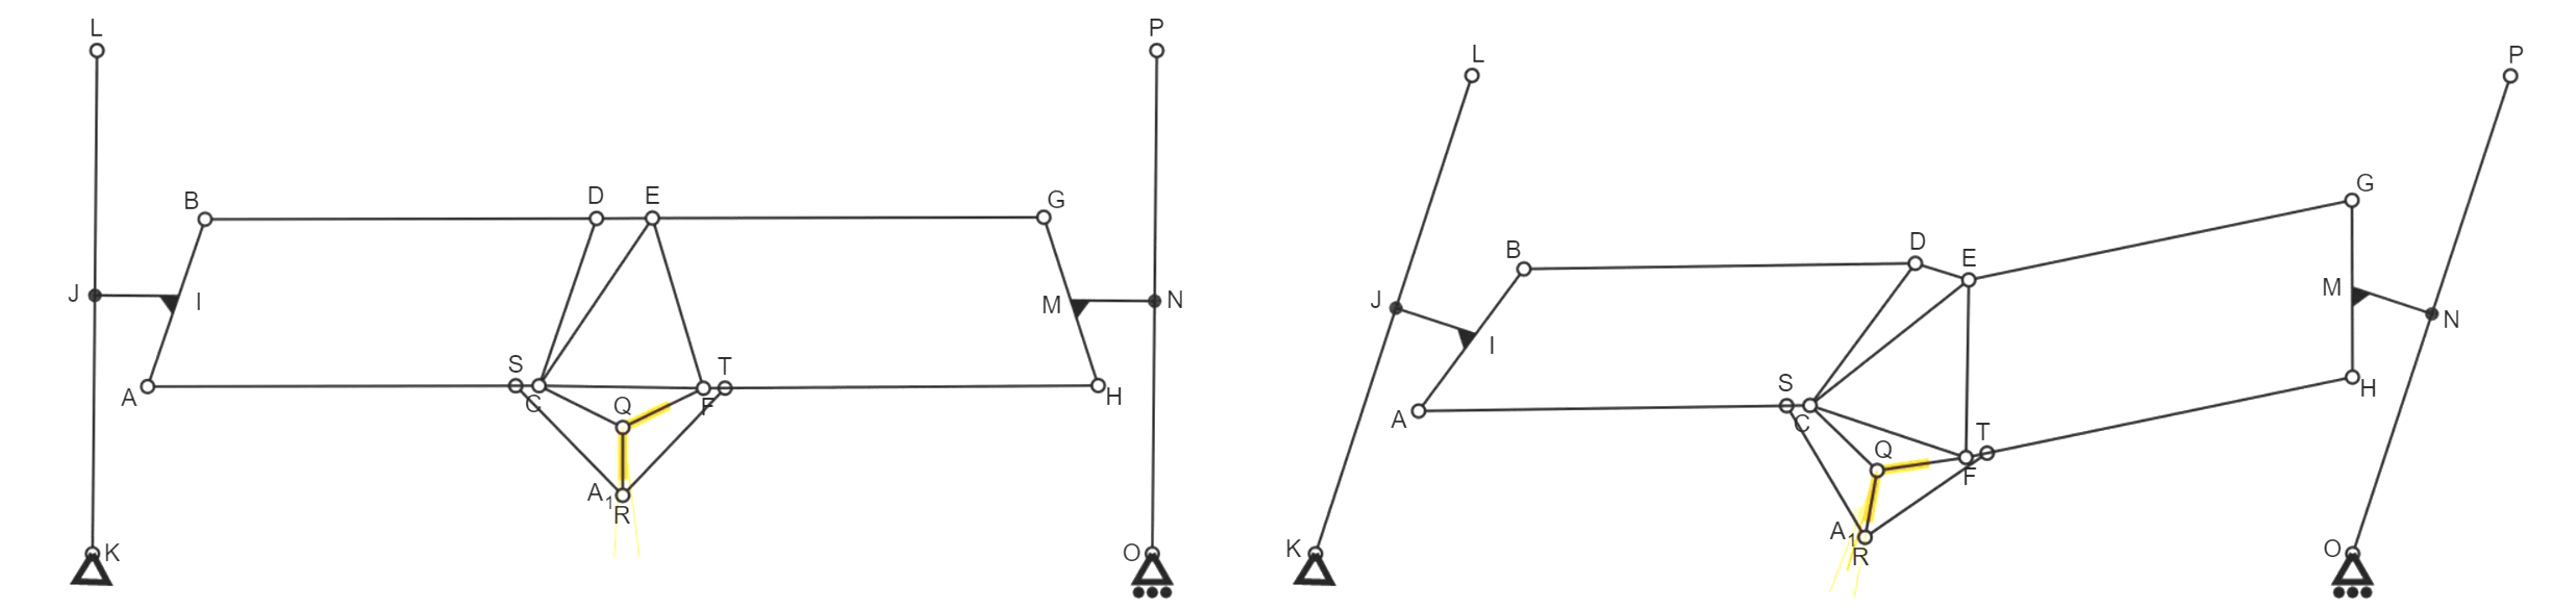
\includegraphics[width=1.1\linewidth]{figs/04/b_2}
		\caption{$B_{2}$ option}
	\end{figure*}
	This strategy is very similar to the B.1, but the motor is located below the body. This can create problems with the motor touching the ground in some circumstances, something that should be avoided. If compared to the previous option, this alternative is not recommended. 
		
		\item \textbf{B.3 Rotating point inside body + horizontal shock absorbers to lower arms}
	
	\begin{figure*}[h!]
		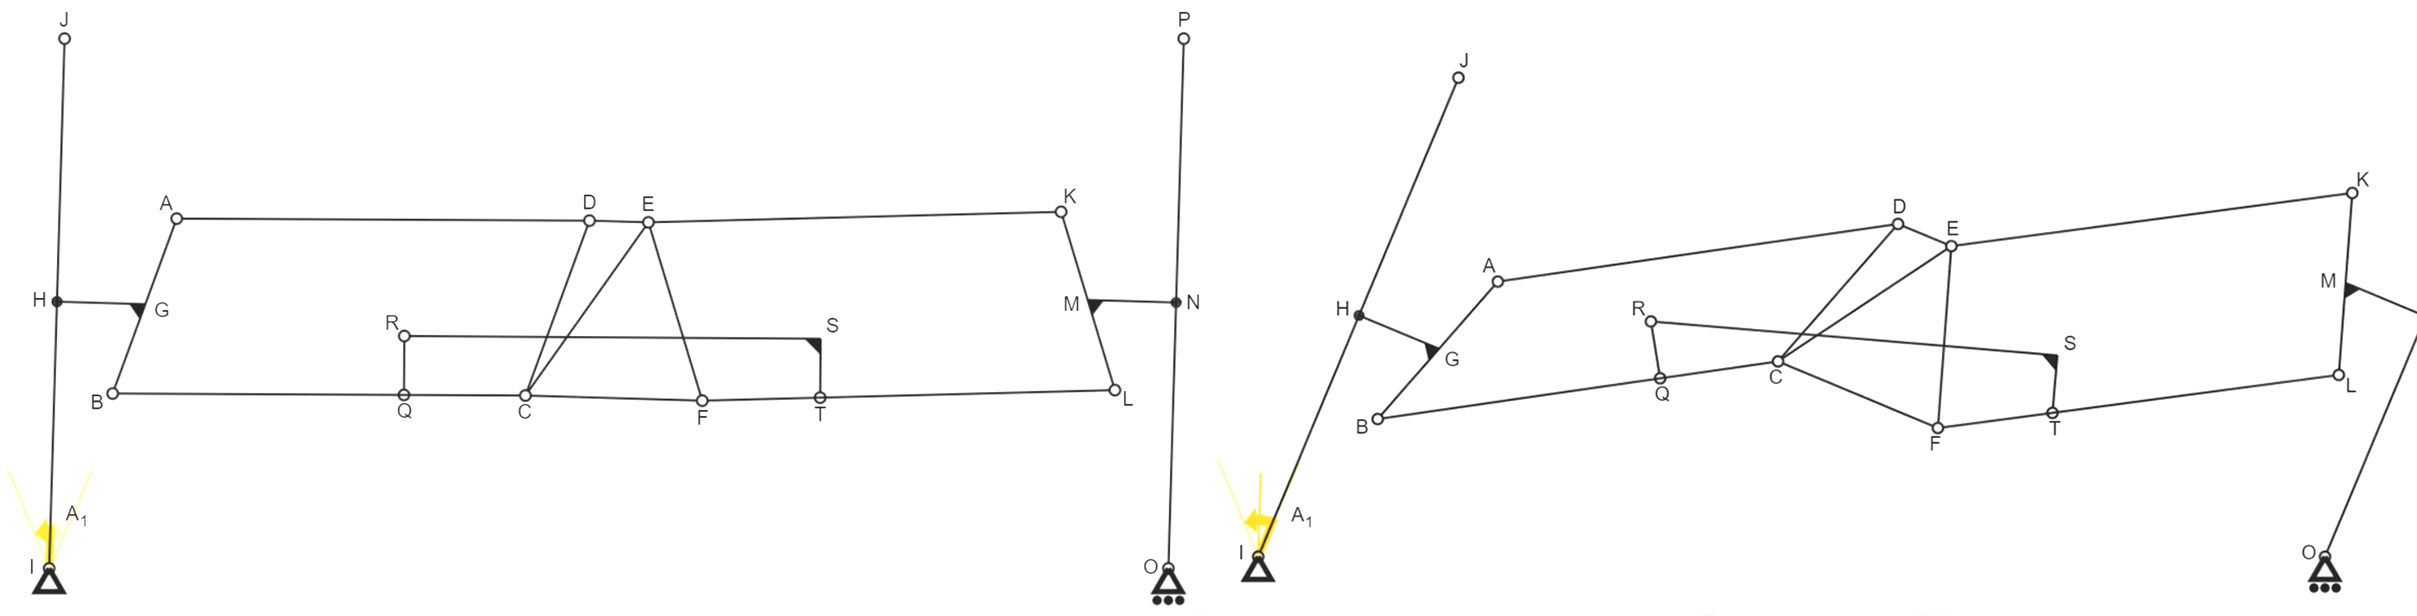
\includegraphics[width=1.1\linewidth]{figs/04/b_3}
		\caption{$B_{3}$ option}
	\end{figure*}
	Using a rotary motor and a rack-pinion system, the rotational motion can be transformed into a linear (horizontal) motion, thus changing the distance between the lower suspension arms and tilting the vehicle.
	
	\newpage
	\item \textbf{B.4 Rotating point inside body + gearbox to lower arm}
	
	By means of a gearbox, the torque coming from the motor is increased, as the suspension arms are actuated art the same time. The simplicity and freedom to choose the reduction ratio were the main reasons why this option was designed, fabricated and assembled in the full scale PEV.
	\begin{figure*}[h!]
		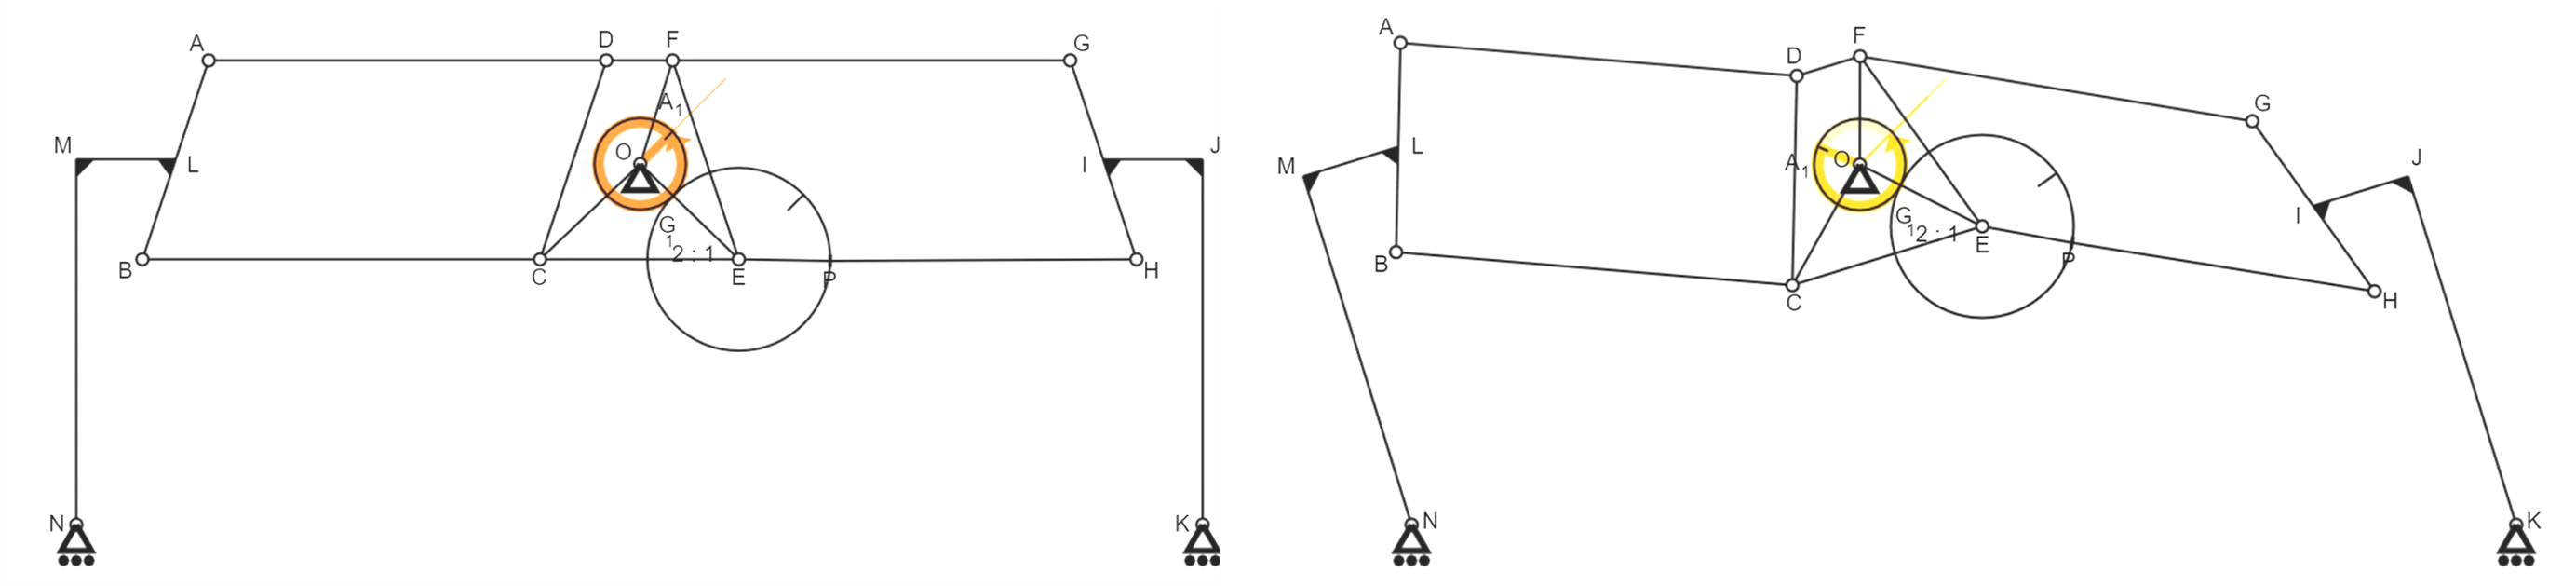
\includegraphics[width=1.1\linewidth]{figs/04/b_4}
		\caption{$B_{4}$ option}
	\end{figure*}
\end{itemize}
\end{itemize}
As has already been stated, the miniPEV will have a tilting mechanism similar to the option B.1 whereas the full scale PEV will be designed following the B.4 design. 

\subsection{First Sketches}

At first, some drawings were made to illustrate the model in three dimensions.
In Figure \ref{sketch_1}, the tilt actuator and the arms with the shock absorbers activate the tilting on the trike. The suspension is constituted by a 4-bar mechanism; the simplest bar system that allows a tilting motion.
\begin{figure}[h!]
	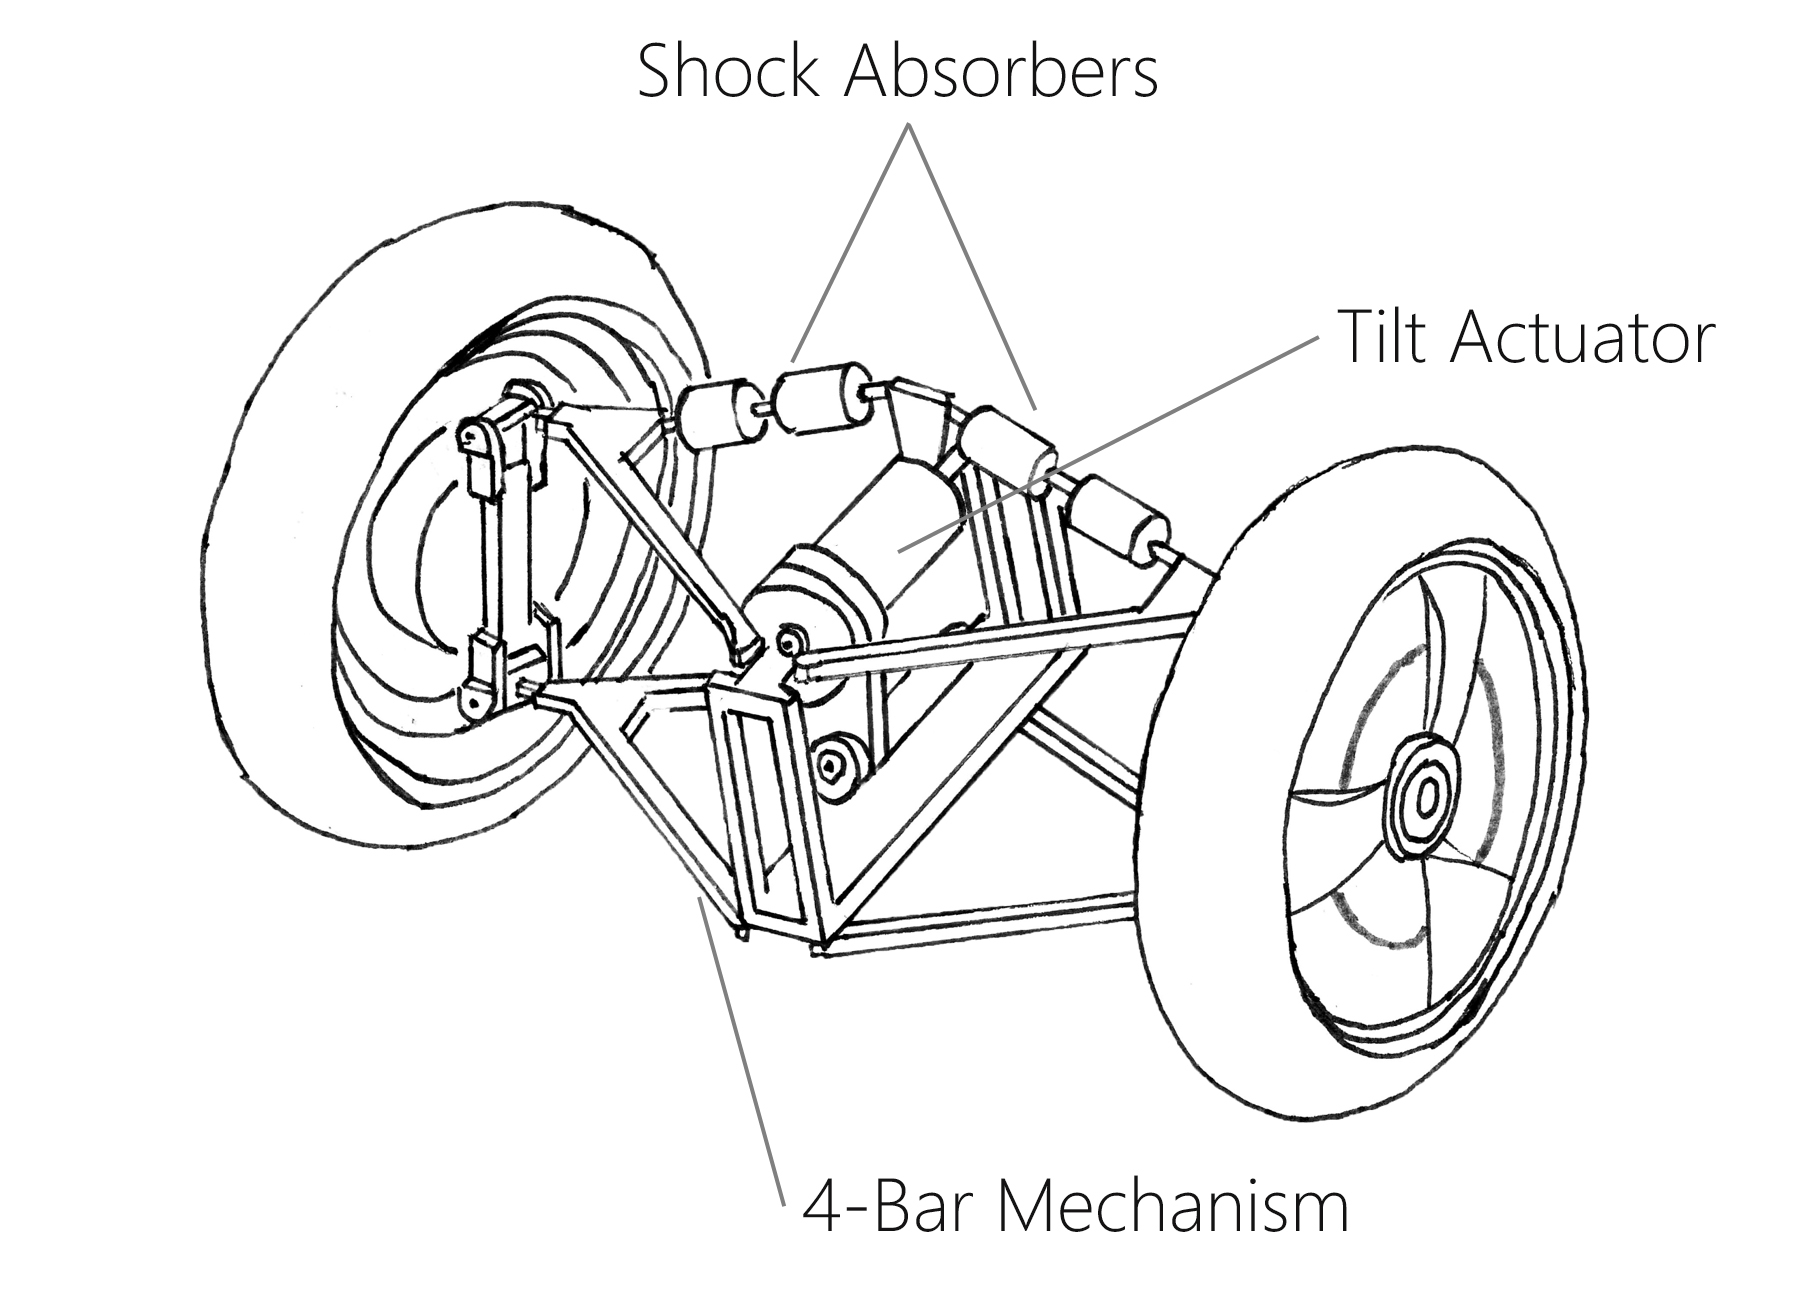
\includegraphics[width=0.95\linewidth]{figs/04/Imagen5}
	\caption{Sketch of tilting mechanism}
	\label{sketch_1}
\end{figure}

The front and rear views of the suspension (Figure \ref{sketch_2}) clarify the 4-bar mechanism mentioned previously. When the vehicle runs into a bump, the shock absorbers in the affected side compress, thus minimizing the vibrations that reach to the driver. In addition, the suspension allows the tilting of the vehicle an angle $\theta$, which will be limited by the geometry, but should not exceed 30 degrees.
\begin{figure*}[h!]
	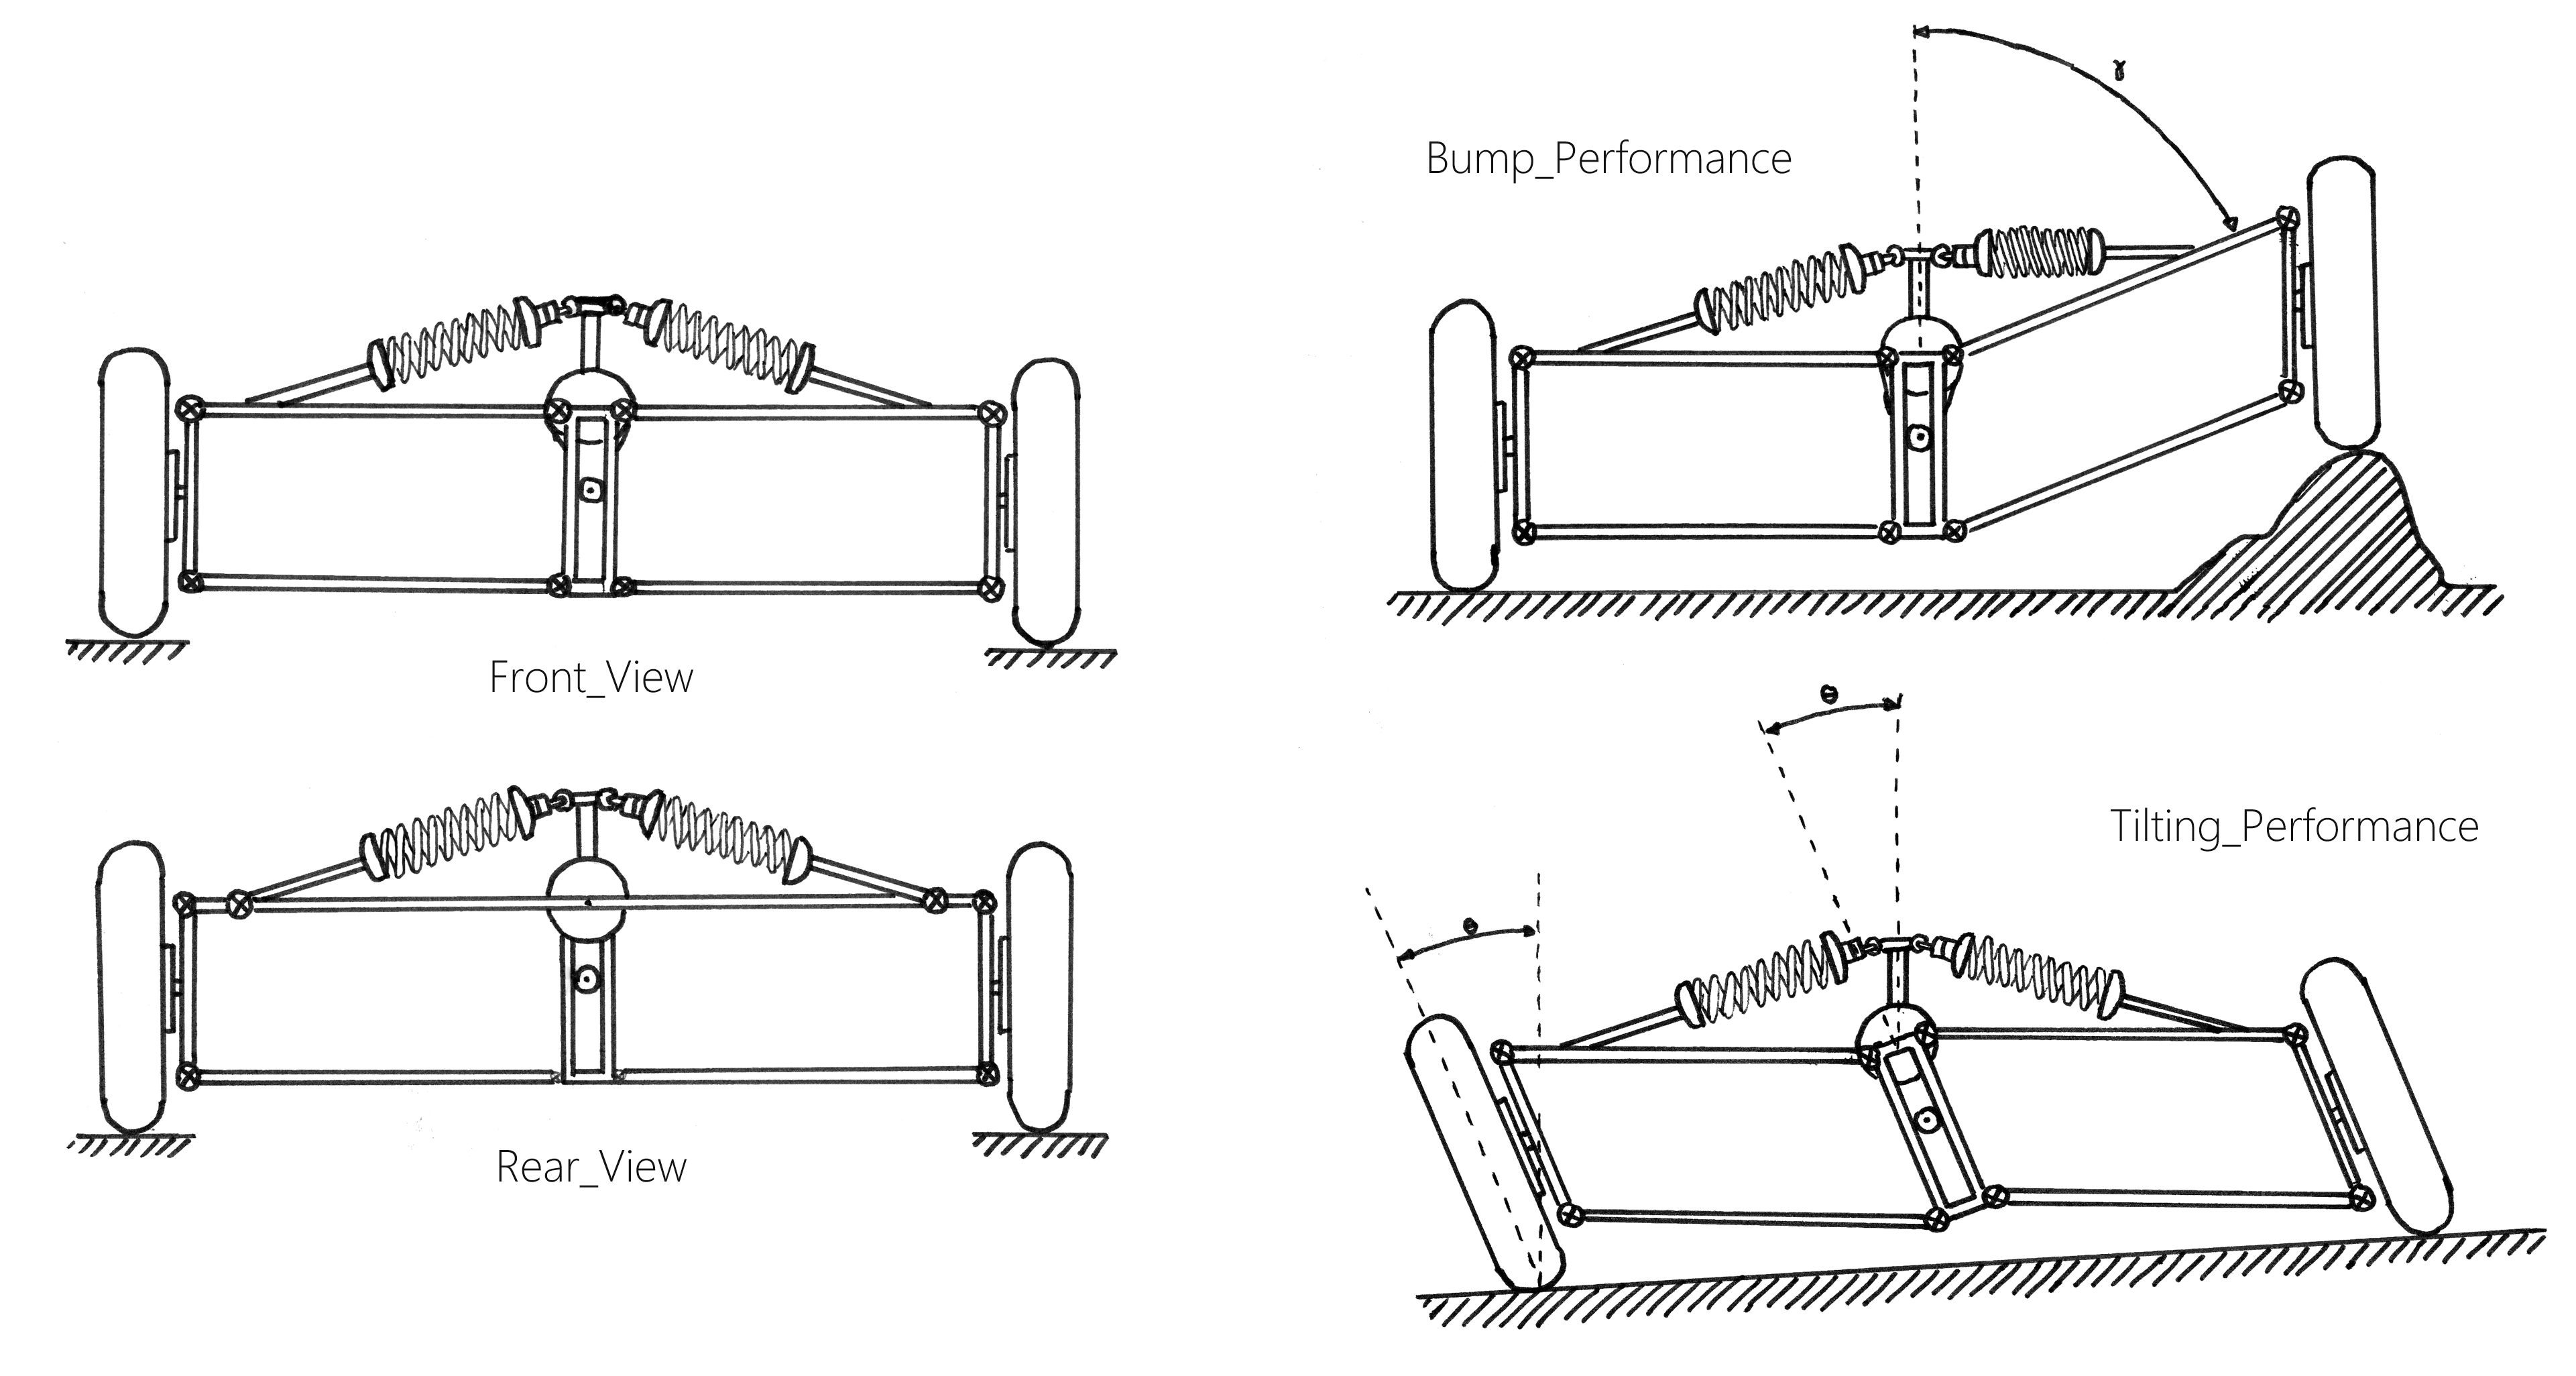
\includegraphics[width=1.0\linewidth]{figs/04/Imagen6}
	\caption{Sketches with response to bump and tilting}
	\label{sketch_2}
\end{figure*}

\\In Figure \ref{sketch_3} more detailed drawings of the suspension have been included.
\begin{figure*}[h!]
	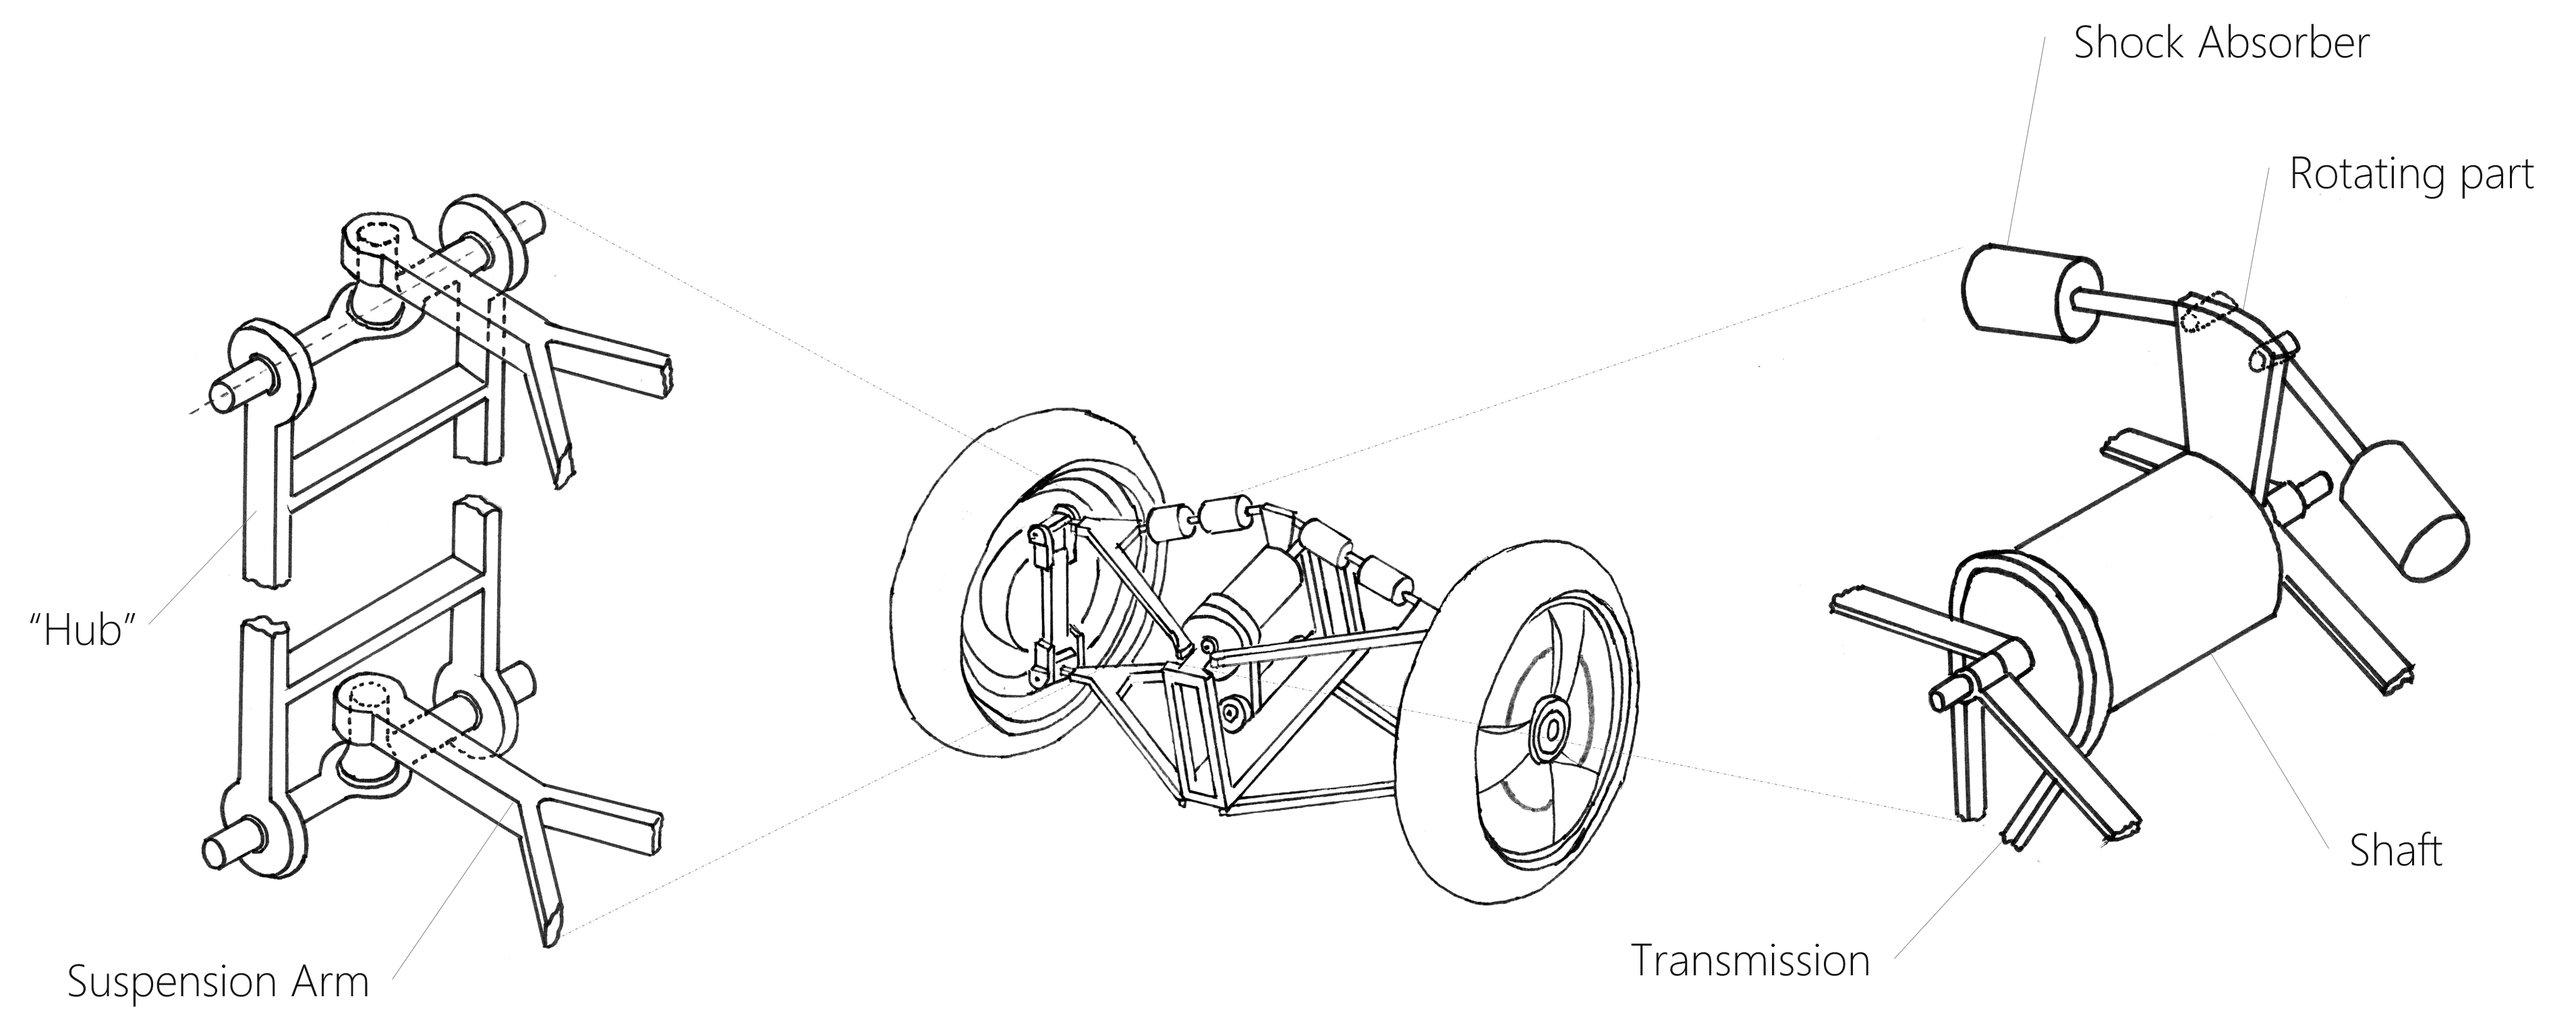
\includegraphics[width=1.0\linewidth]{figs/04/Imagen10}
	\caption{Detailed sketches of the tilting suspension}	
	\label{sketch_3}
\end{figure*}

\newpage
\section{Components}

In this section the components of the miniPEV and their main characteristics are reviewed.

\begin{figure}[h!]
	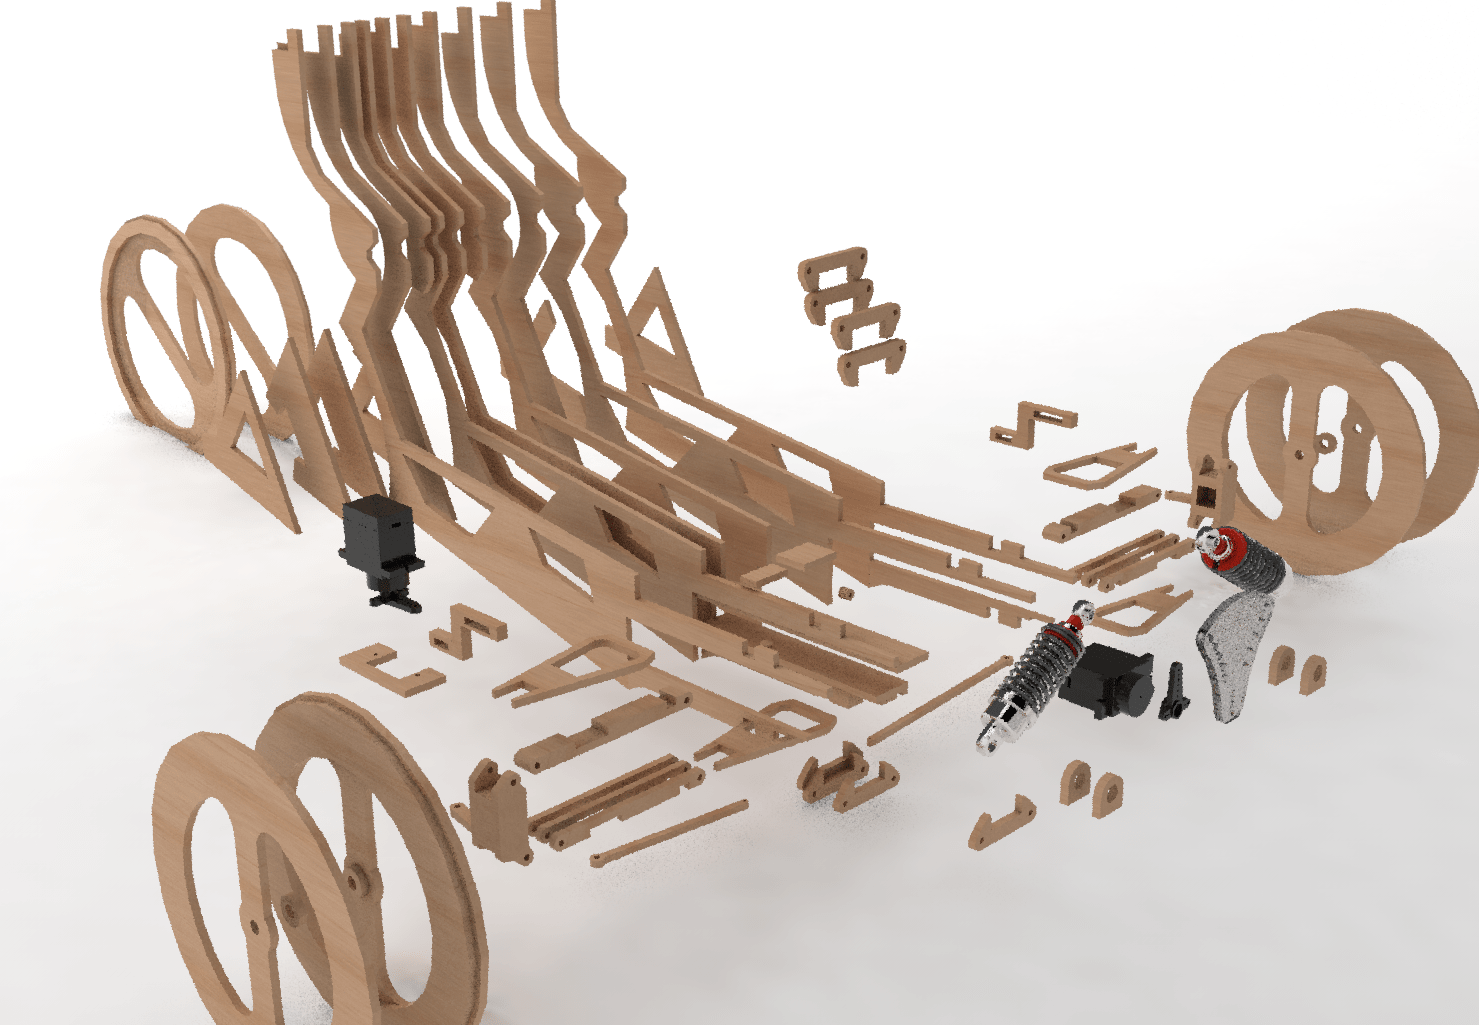
\includegraphics[width=0.95\linewidth]{figs/04/CreamBoxtemp0150}
	\caption{miniPEV explosion render}
\end{figure}
%\begin{figure}[h!]
%	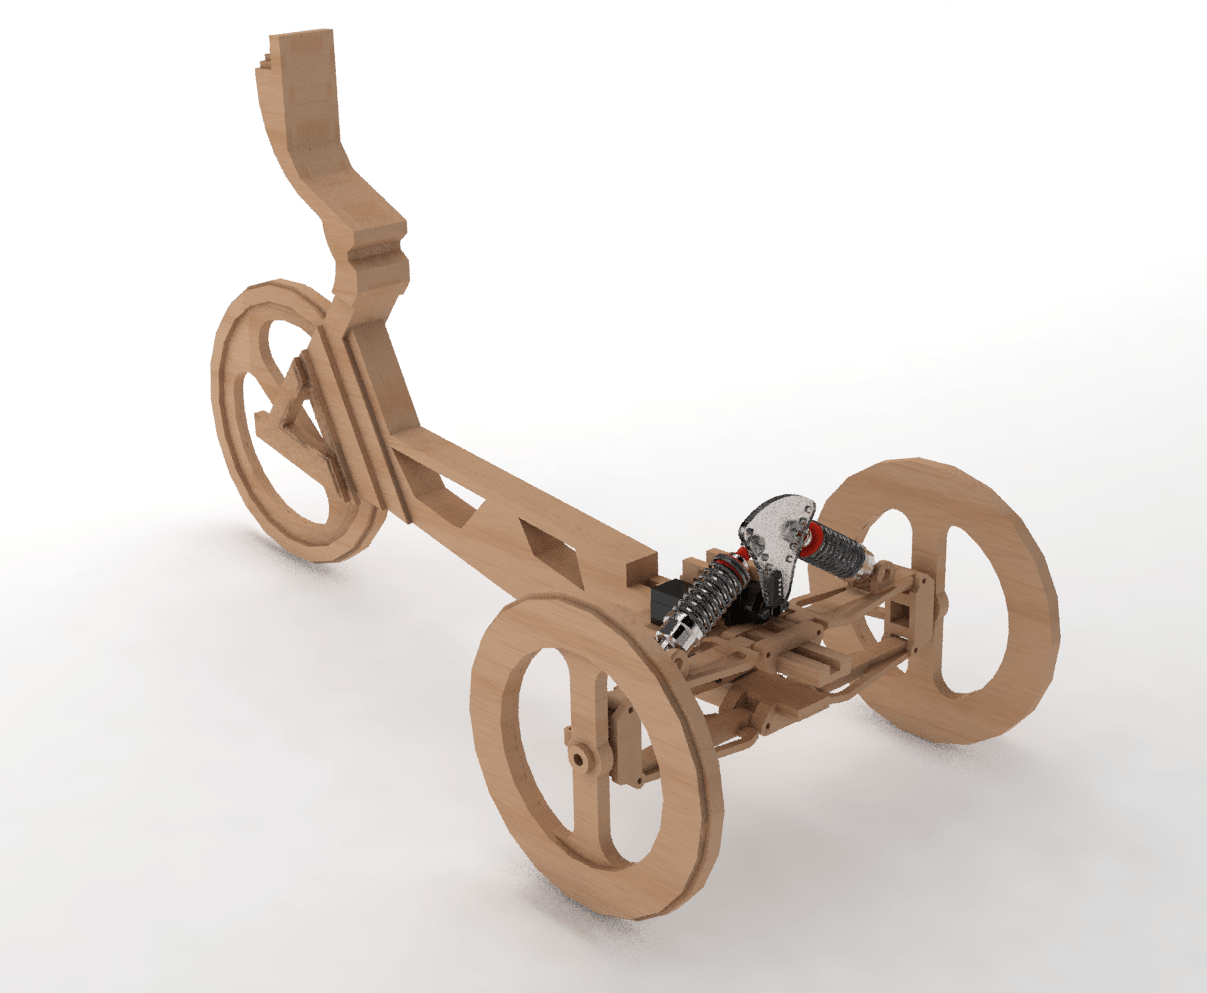
\includegraphics[width=1.0\linewidth]{figs/04/CreamBoxtemp0210}
%	\caption{miniPEV render}
%\end{figure}
\begin{itemize}
\begin{itemize}
	\item Wood Frame and Wheels
	
	Taking as example other previous wood models from the group, the vehicle was designed in Solidworks. The body is made of 3mm plywood sheets, and the rear wheel is slightly bigger than the front ones. Using the laser cutting machine, the body, the wheels, and the rest of the parts were fabricated quite fast. The fact that the model was made out of plywood brought along a lot of issues during the motion of the vehicle. This type of prototypes are not usually designed to move, but to remain static instead. In any case, there was a lot of effort in reducing the friction between the moving parts (wheels and steering system).
	
	\begin{figure}[h!]
		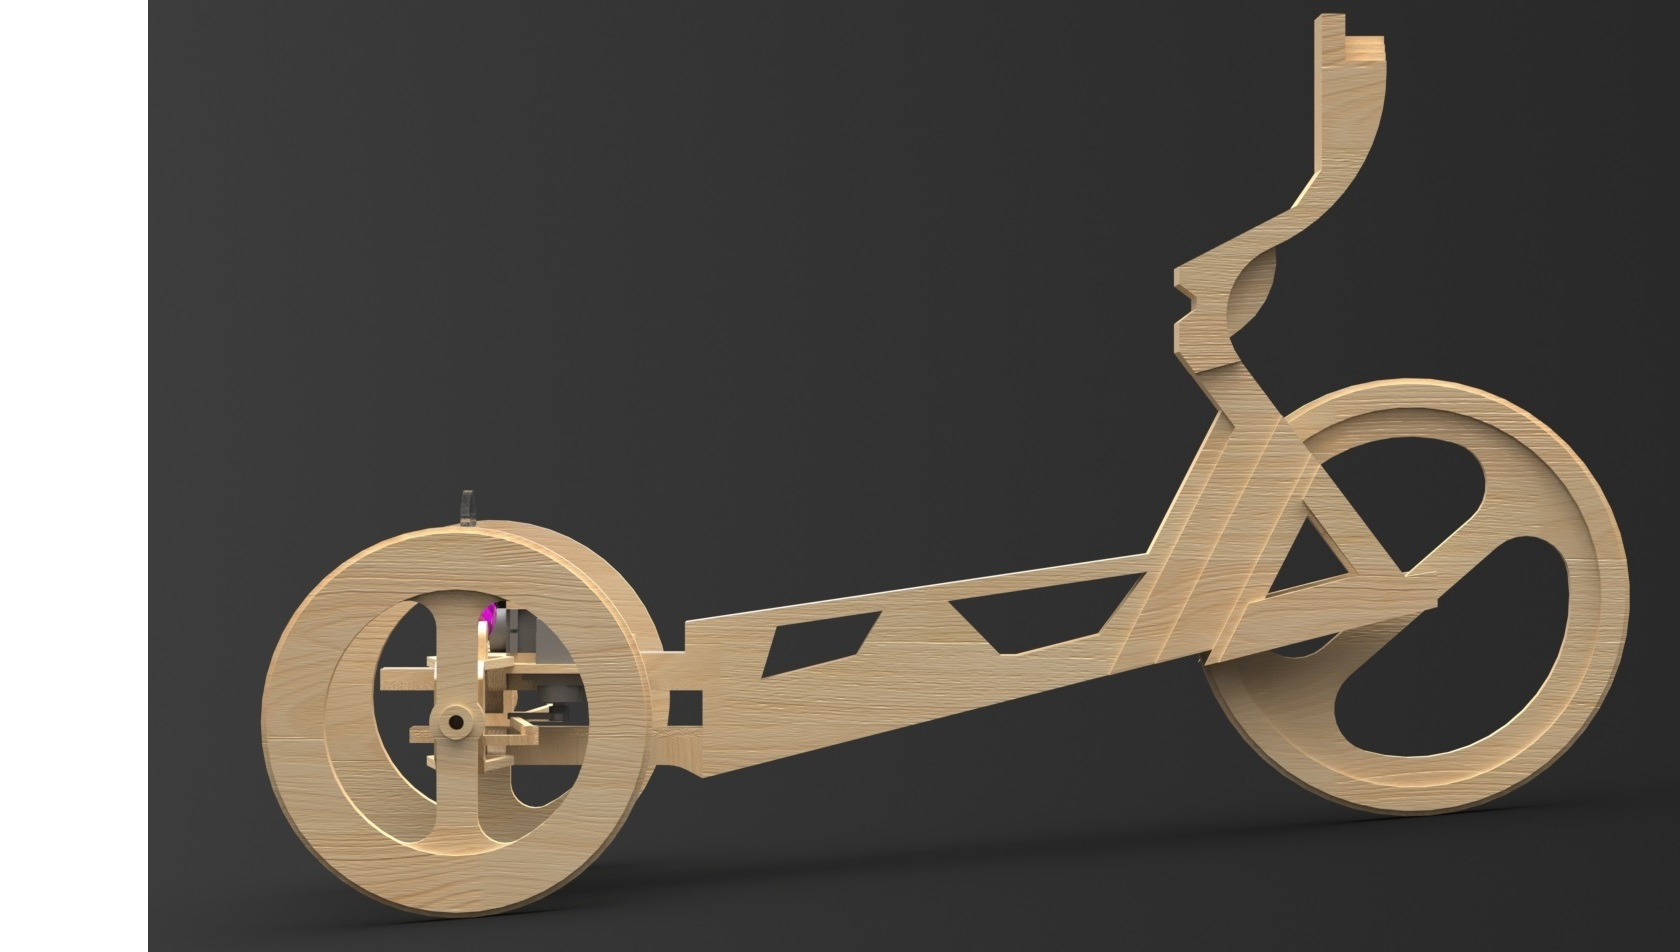
\includegraphics[width=1.0\linewidth]{figs/04/11}
		\caption{Lateral view of the render}
	\end{figure}
	
	\newpage
	\item Rear DC Motor
	
	The rear motor is a Pololu DC motor of 12V and a gearbox integrated. The gearbox fits perfectly in this application, providing a high output torque to be able to move the vehicle. The torque increase is about 50:1, and the motor's small size allows it to hide in the frame.
	\begin{marginfigure}[-2cm]
		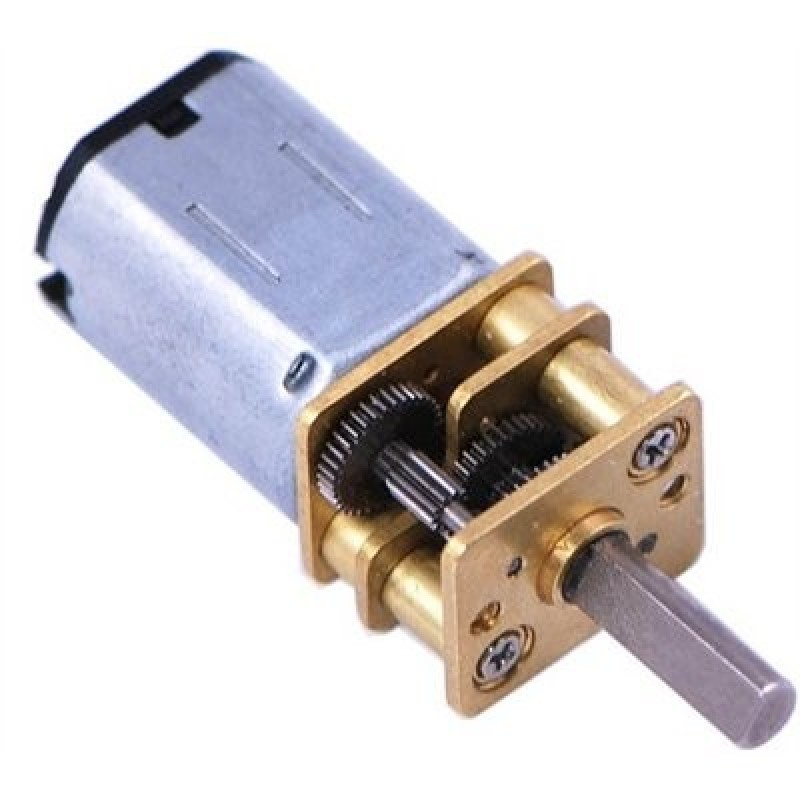
\includegraphics[width=0.75\linewidth]{figs/04/pololu}
		\caption{Rear DC Motor, Pololu 50:1 Micro Metal Gearmotor }
	\end{marginfigure}
	
	Controlling a DC motor with Arduino requires a transistor and a diode. The small DC motor is likely to use more power than an Arduino digital output can handle directly (50mA). Connecting the motor straight to an Arduino pin would damage the Arduino. Tha is why a small transistor like the PN2222 needs to be used as a switch, that uses just a little current from the Arduino digital output to control the much bigger current of the motor. 

There is also a diode connected across the connections of the motor. Since diodes only allow electricity to flow in one direction, when to motor turns off the diode protect the Arduino and the transistor from a negative spike of voltage. The diode protects against this, by shorting out any such reverse current from the motor.
	
	\item Steering and Tilting	
	
	The steering servo motor is located vertically in the left side of the vehicle, and has two bars linked to the hubs of the front wheels. The tilting motor is laying on top of the body, horizontally, and has a glass arm attached to the output shaft. This glass piece is connected to the shock absorbers that are attached to the upper suspension arms. 
	
	The tilting servo motor is slightly more powerful than the steering motor, since the force requirement for the tilting motion is higher than for turning the wheels.
	
	\begin{marginfigure}[-13cm]
		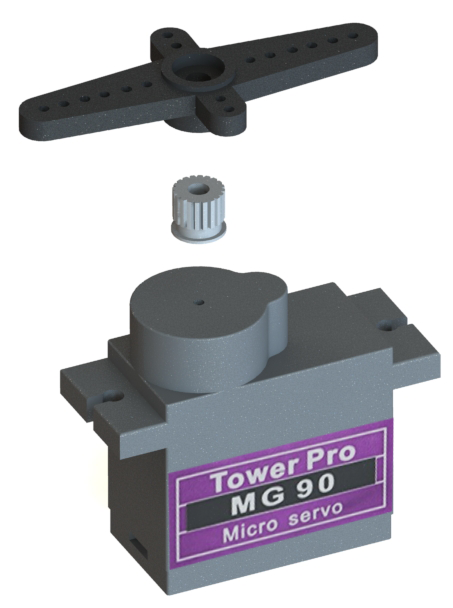
\includegraphics[width=0.75\linewidth]{figs/04/servo}
		\caption{Servo Motor MG90}
	\end{marginfigure}
	
	\begin{marginfigure}[-4cm]
		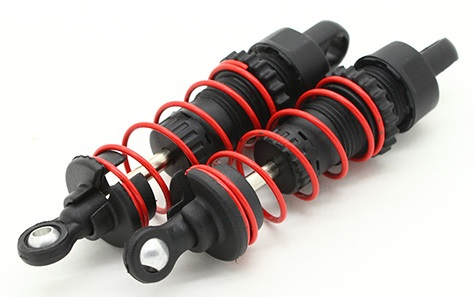
\includegraphics[width=0.85\linewidth]{figs/04/55758}
		\caption{Miniature shock absorbers MA 35 to MA 900}
	\end{marginfigure}
	
	\begin{figure}[h!]
		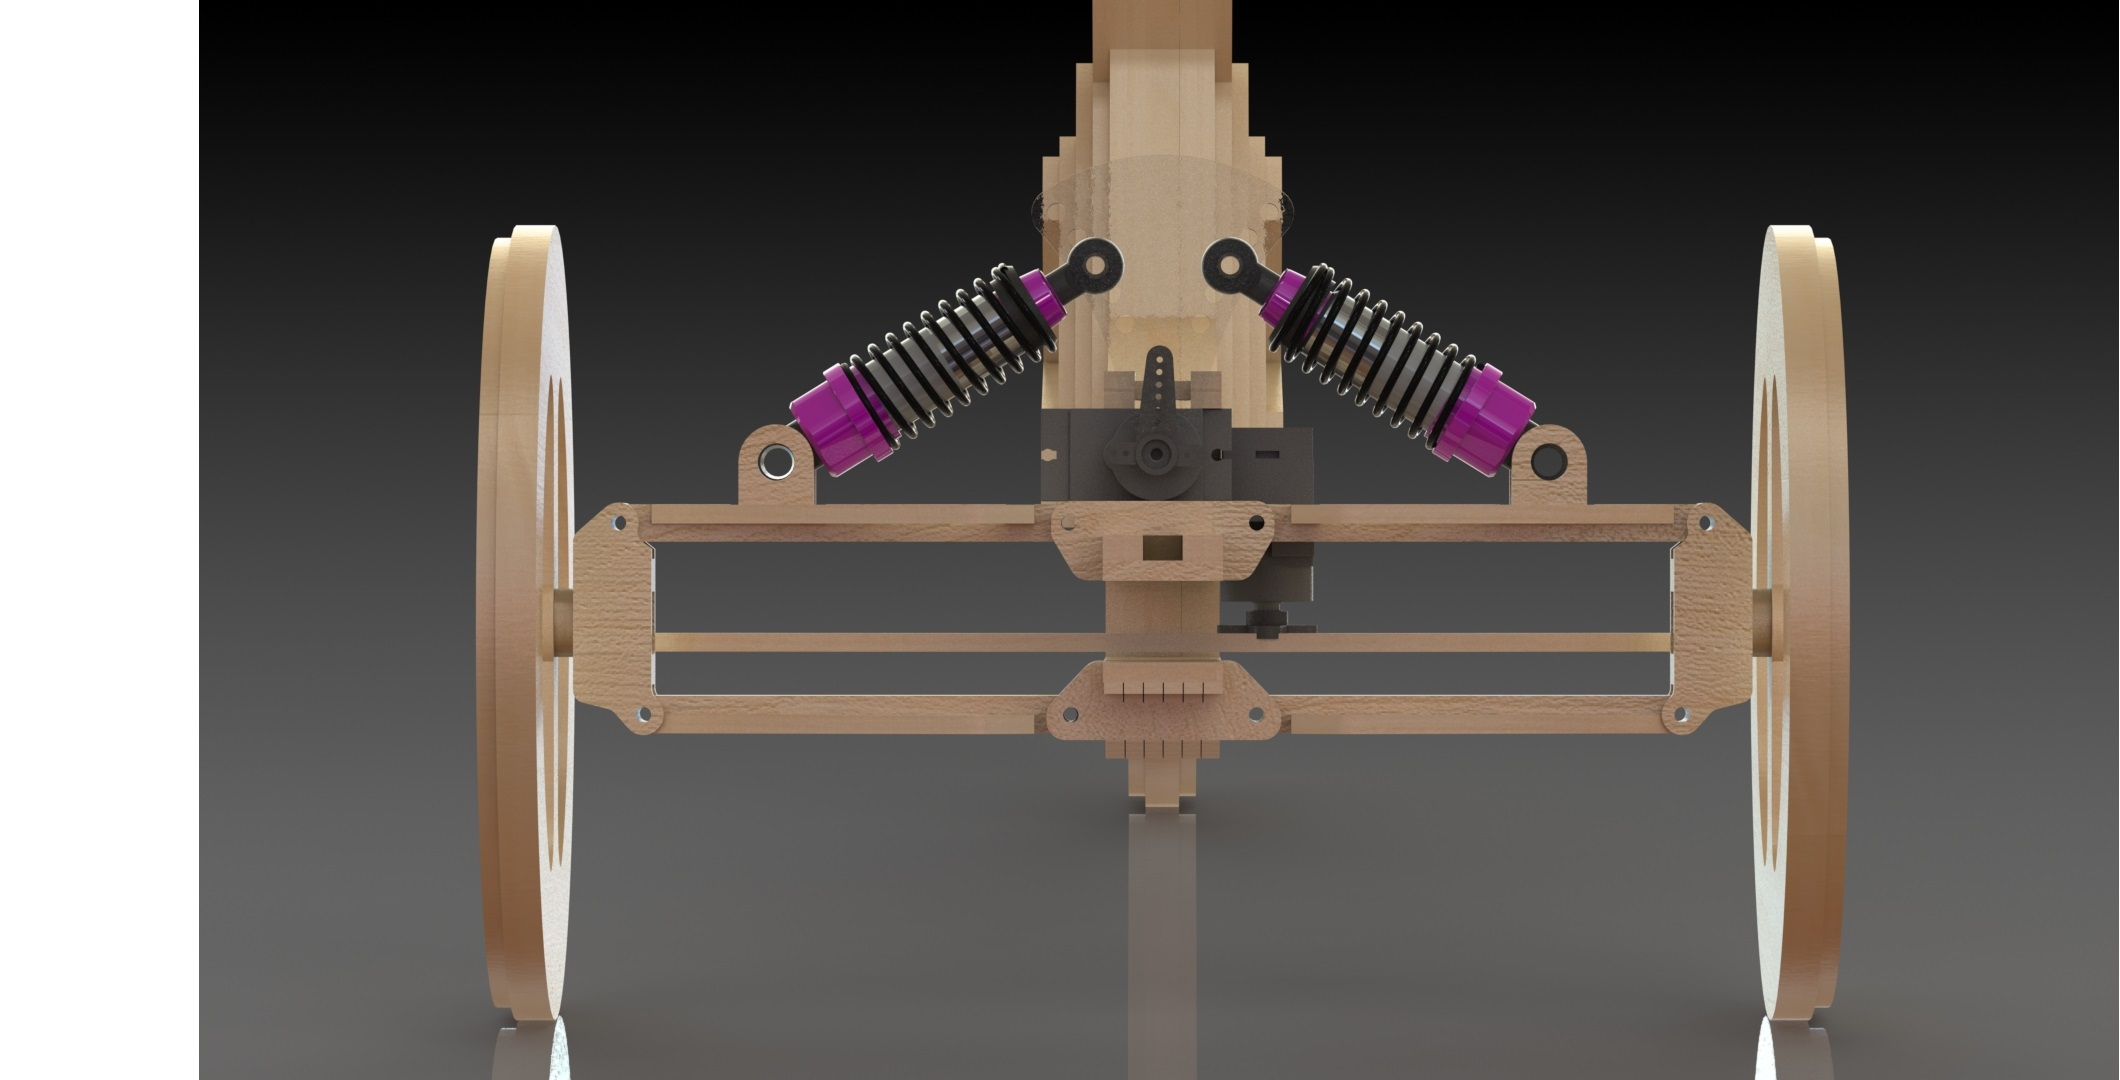
\includegraphics[width=0.95\linewidth]{figs/04/22}
		\caption{Front view of the render}
	\end{figure}

	\item Electronics
	
	The \textbf{Arduino UNO} is the board responsible for receiving the inputs from the sensors and controlling the output to the three motors. The board and all the components are powered by a 12V DC battery (\textbf{Energizer XP8000}). The election of the 12V is due to the rear motor input voltage. The rest of the components (servo motors, bluetooth module and IMU) only require 5V, voltage that the Arduino board can provide from one of its pins. All these electronic components are placed in a mini breadboard.
	
	The chosen IMU both for the miniPEV and for the PEV is the \textbf{Adafruit BNO055 Absolute Orientation Sensor}, with 9DOF (accelerometer, gyroscope and magnetometer). It is connected through the I2C connection (SDA and SCL pins) to the board. The measurements from this sensor are the angular velocity along the vertical axis $Z$ (\textbf{yaw rate} $\dot{\psi}$) and the \textbf{linear acceleration} in the forward direction $a_{x}$, which will be integrated to estimate the longitudinal speed of the vehicle.
	
	As a matter of fact, the use of this Inertial Measurement Unit is quite easy, since the libraries to get the data have been already developed. Nevertheless, there are some steps that need to be followed in order to configure the sensor in the first place (this will be intensively explained in the next chapter).
	
	\hfill
	
	\begin{marginfigure}
		\caption{Electronic Components}
	\end{marginfigure}
	\begin{figure}[!h]
		\minipage{0.5\textwidth}%
			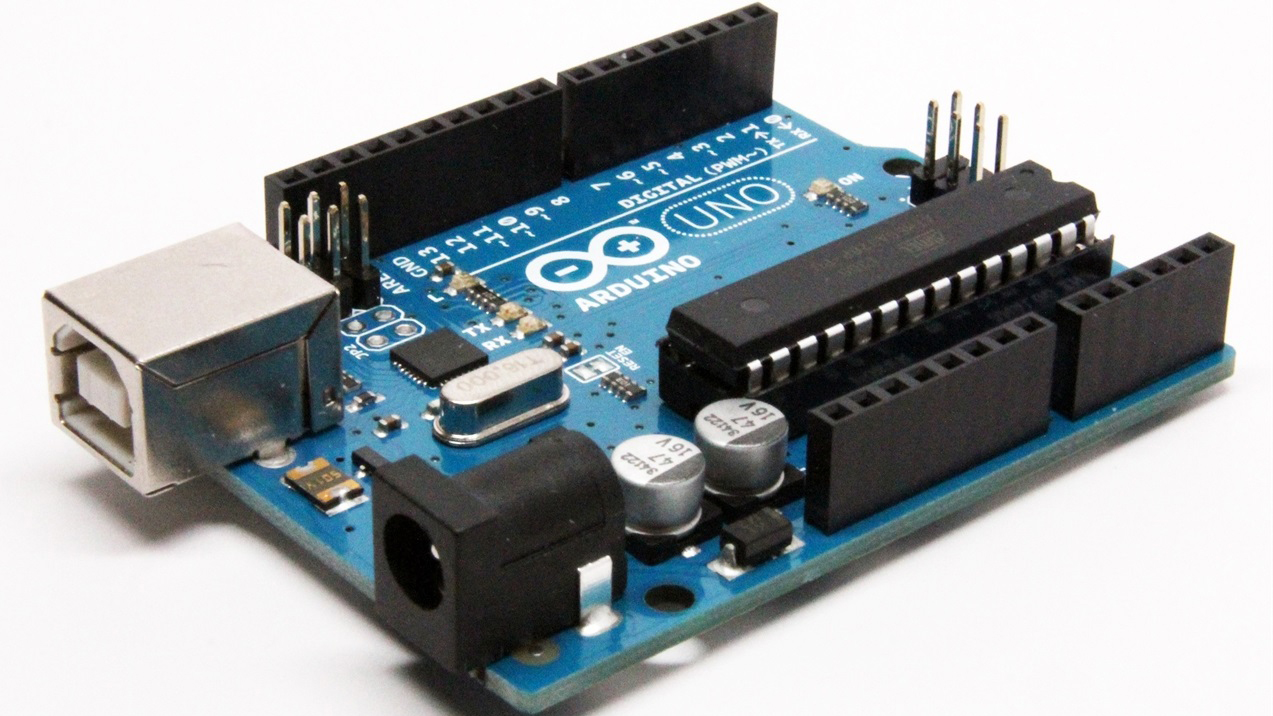
\includegraphics[width=1.0\linewidth]{figs/04/uno}
			\captionof{a)}{ Arduino UNO board}
		\endminipage
		\minipage{0.5\textwidth}
			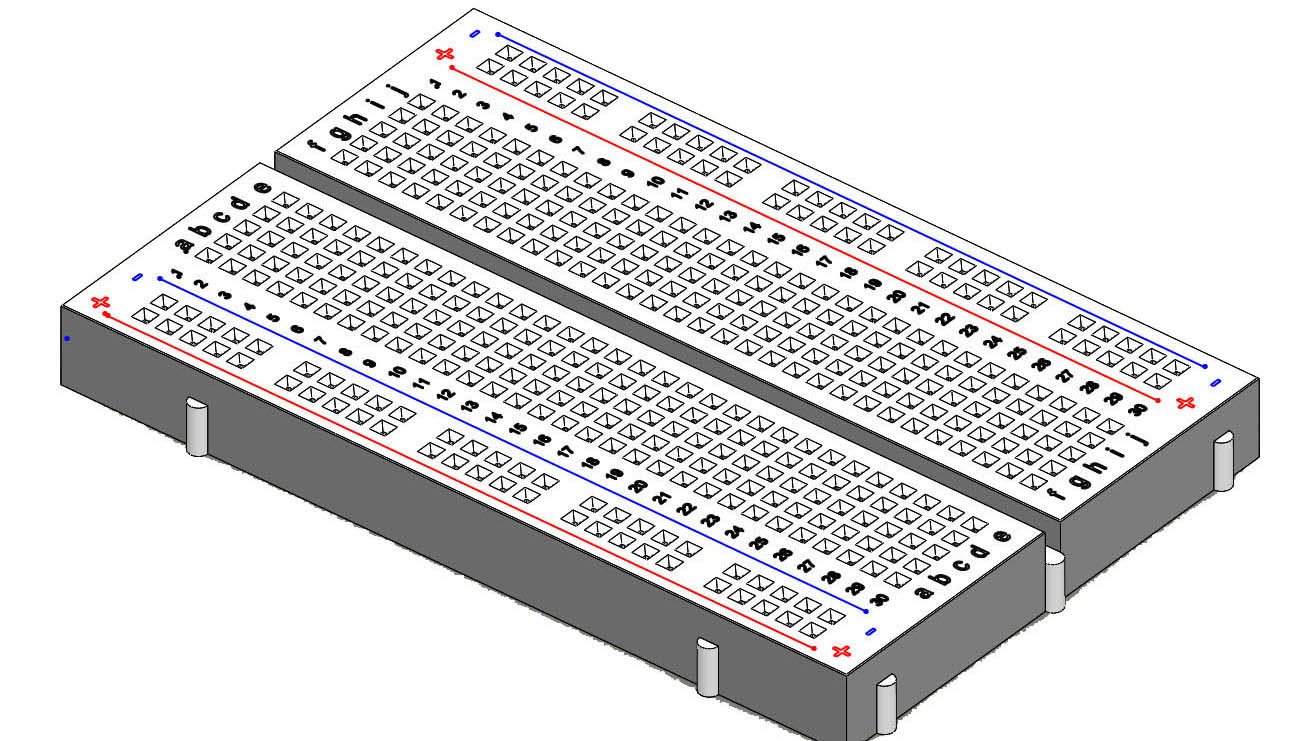
\includegraphics[width=1.0\linewidth]{figs/04/MiniBreadBoard}
		    \captionof{b)}{ Mini breadboard}
		\endminipage\hfill
	\end{figure}
	
	\hfill
	
	\begin{figure}[!h]
		\minipage{0.5\textwidth}
			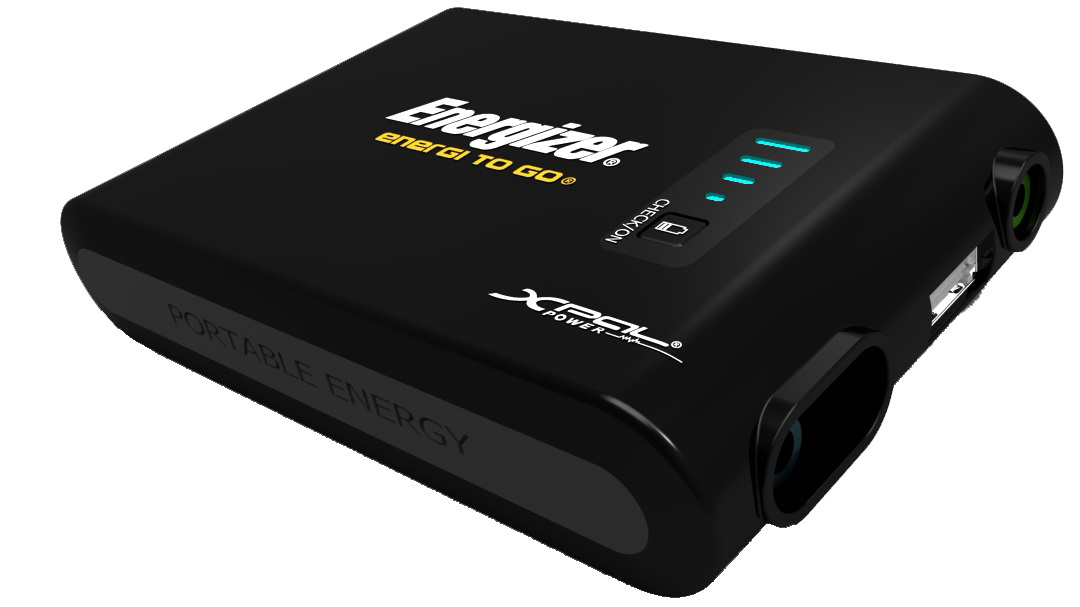
\includegraphics[width=1.0\linewidth]{figs/04/battery}
		  	\captionof{c)}{ Energizer XP8000 battery}
		\endminipage\hfill
		\minipage{0.5\textwidth}
			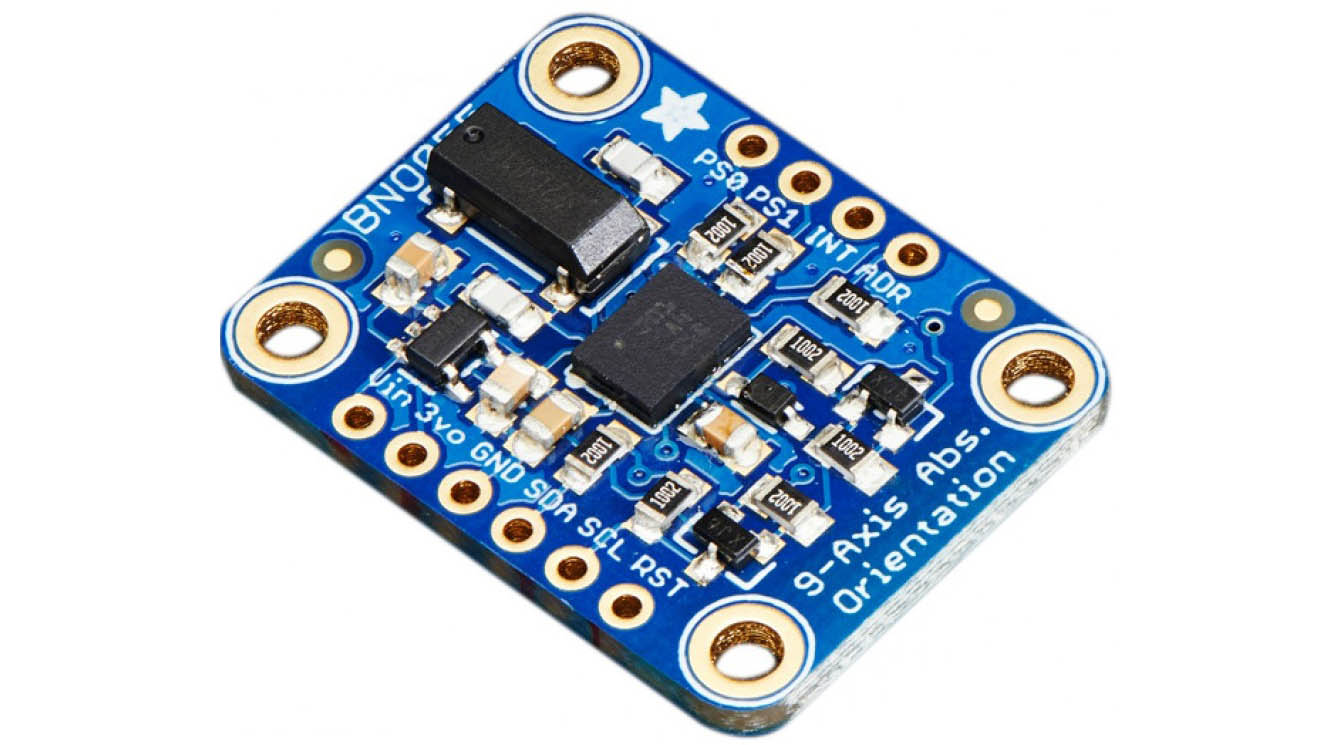
\includegraphics[width=1.0\linewidth]{figs/04/bno055}
		    \captionof{d)}{ BNO055 9DOF IMU}
		\endminipage\hfill
	\end{figure}

	\newpage
	Finally, in order to remotely connect with the board and control the vehicle, a Bluetooth HC05 module was installed. This module was connected through serial connection to the Arduino. An Android application was the installed in the phone to activate different functions (forward, left, right...). The wiring diagram is represented as follows:
	
	\begin{figure*}[h!]
		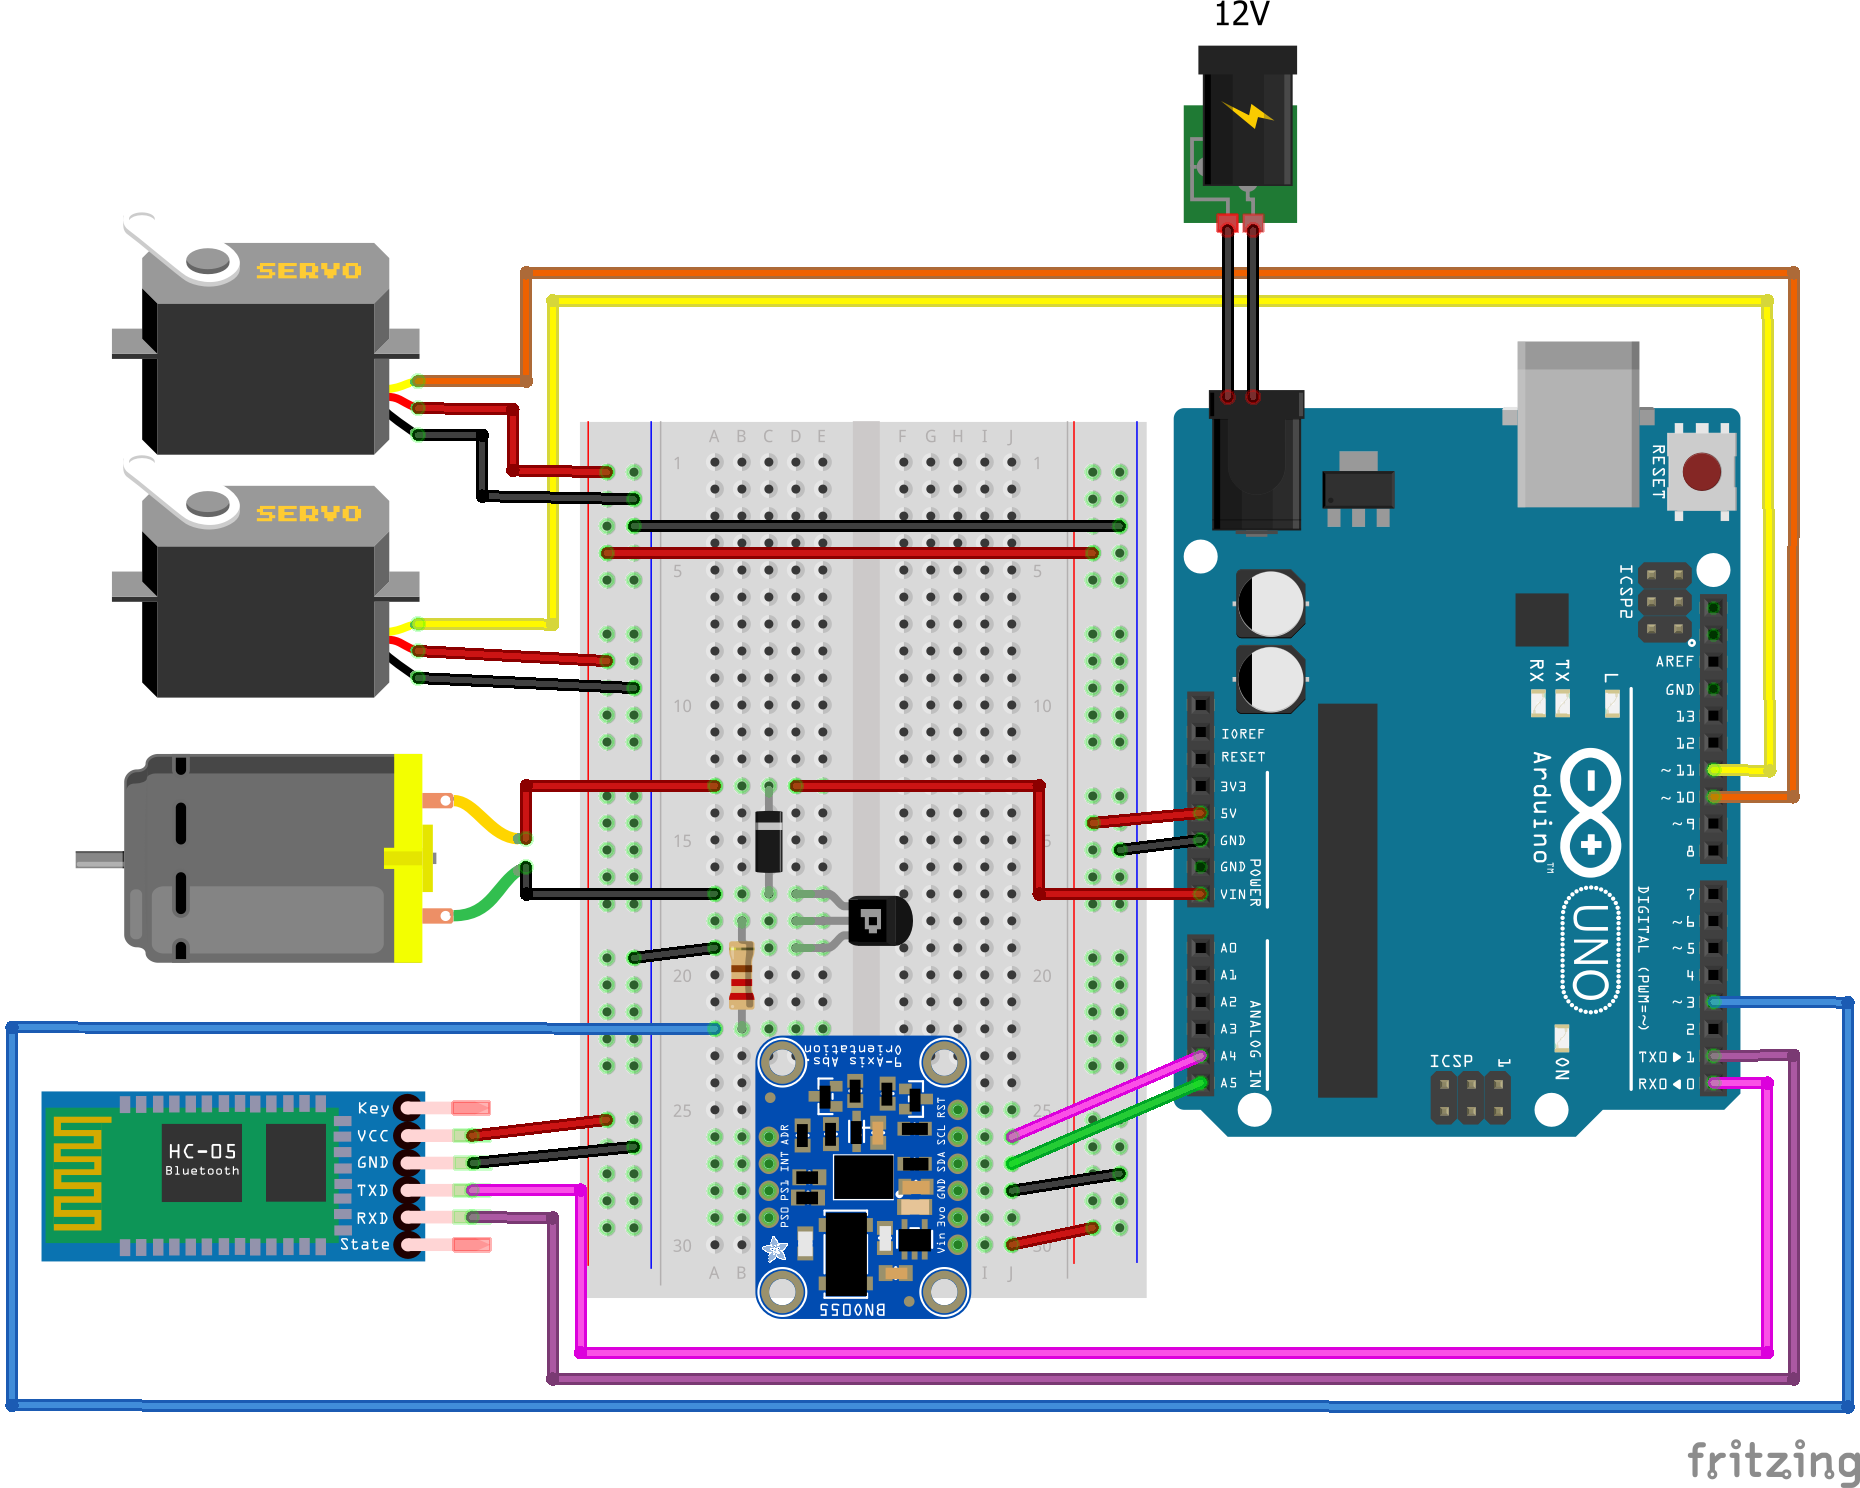
\includegraphics[width=0.9\linewidth]{figs/04/miniPEV_bb}
		\caption{miniPEV Electronics Schematic}
	\end{figure*}

	
\end{itemize}
\end{itemize}
\hfill

\section{Final Model and Results}

The final model is illustrated in the Figures \ref{minipev1} and \ref{minipev2}. The tilting servo motor is controlled to satisfy in every moment that $\theta=\theta_{ref}$, with \[\theta_{ref}=\frac{V\,\dot{\psi}}{g}\] This expression of the roll angle reference was introduced in the previous chapter and is based on a very simple model that combines the bicycle and the inverted pendulum dynamics (Figure \ref{miniPEV_model}).

\begin{marginfigure}[-3cm]
	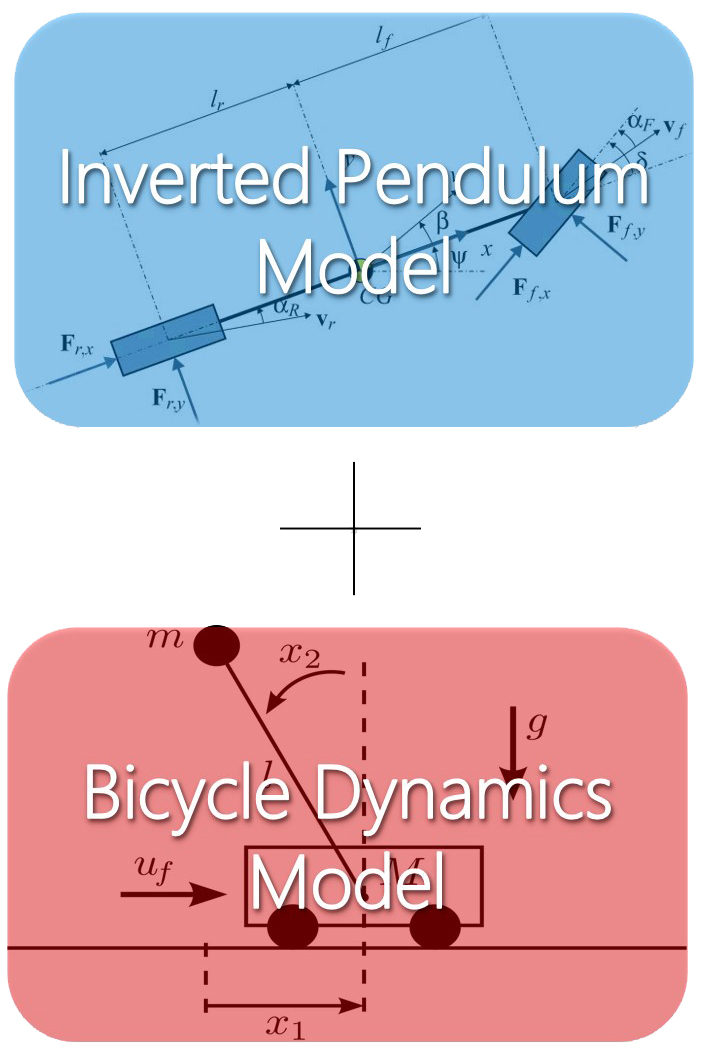
\includegraphics[width=0.75\linewidth]{figs/04/Imagen2}
	\caption{miniPEV simple model to obtain the $\theta_{ref}$}
	\label{miniPEV_model}
\end{marginfigure}

\begin{figure}[h!]
	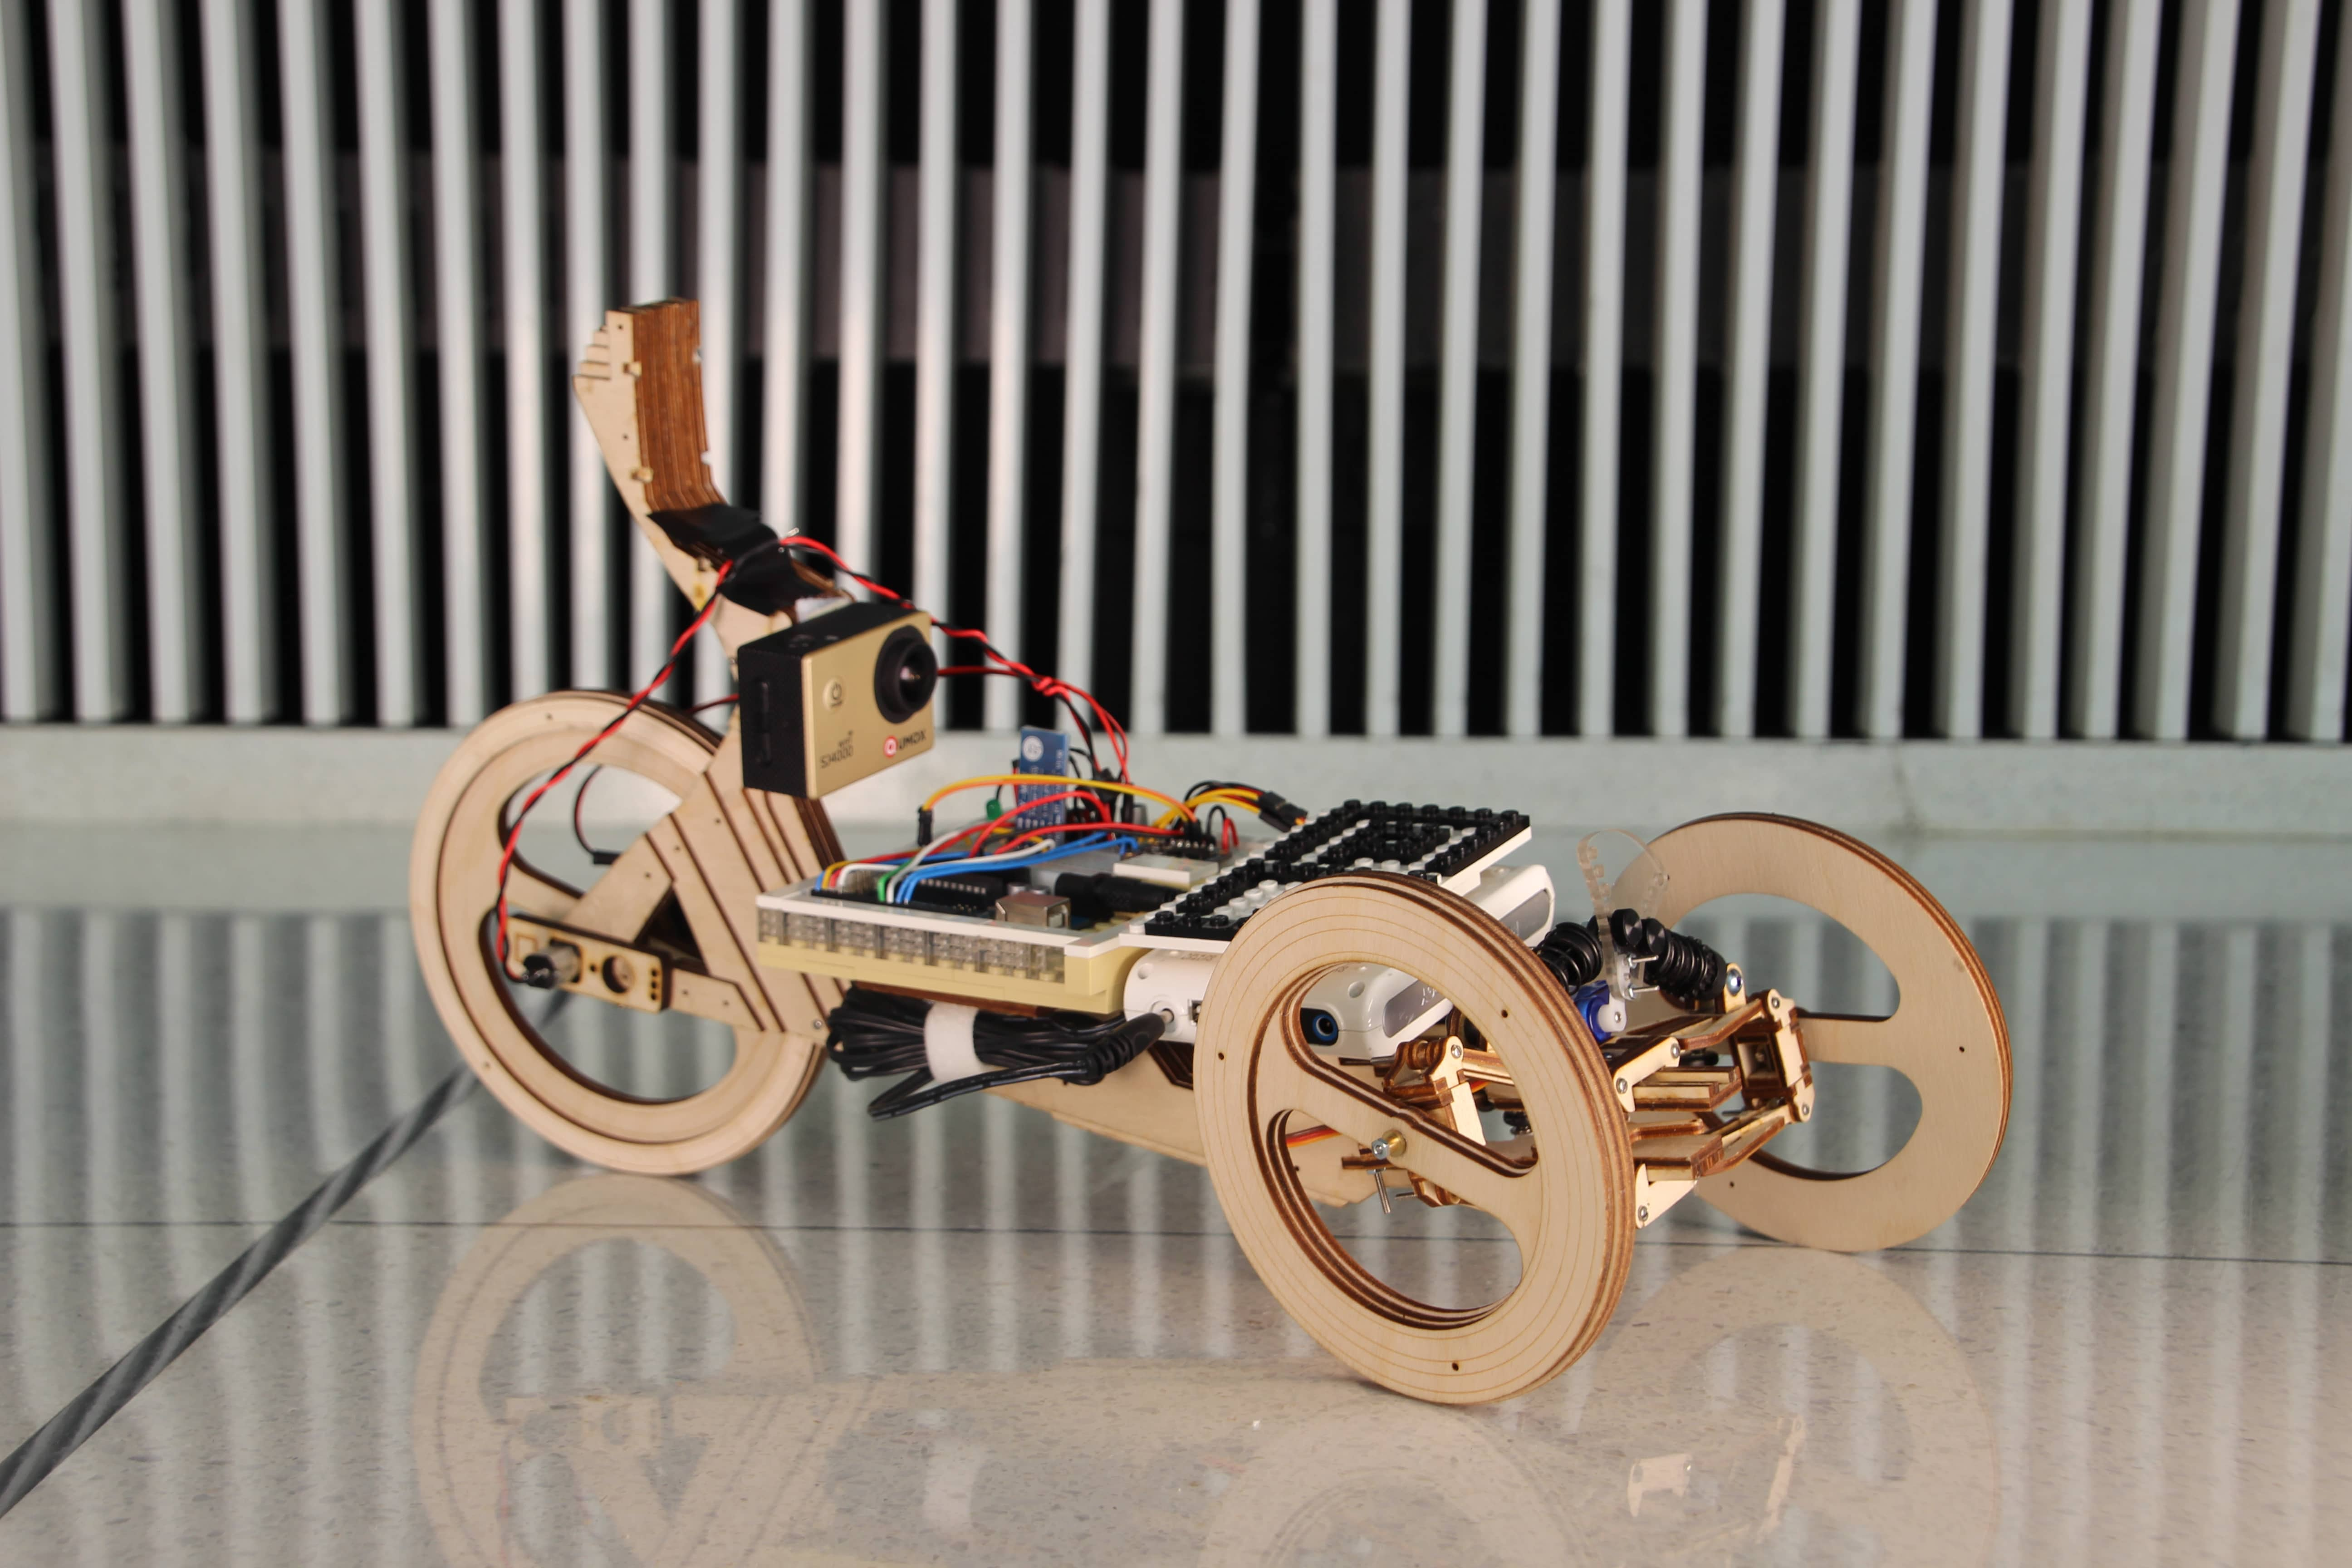
\includegraphics[width=1.0\linewidth]{figs/04/IMG0943}
	\caption{Lateral view of the miniPEV}
	\label{minipev1}
\end{figure}

\begin{figure}[h!]
	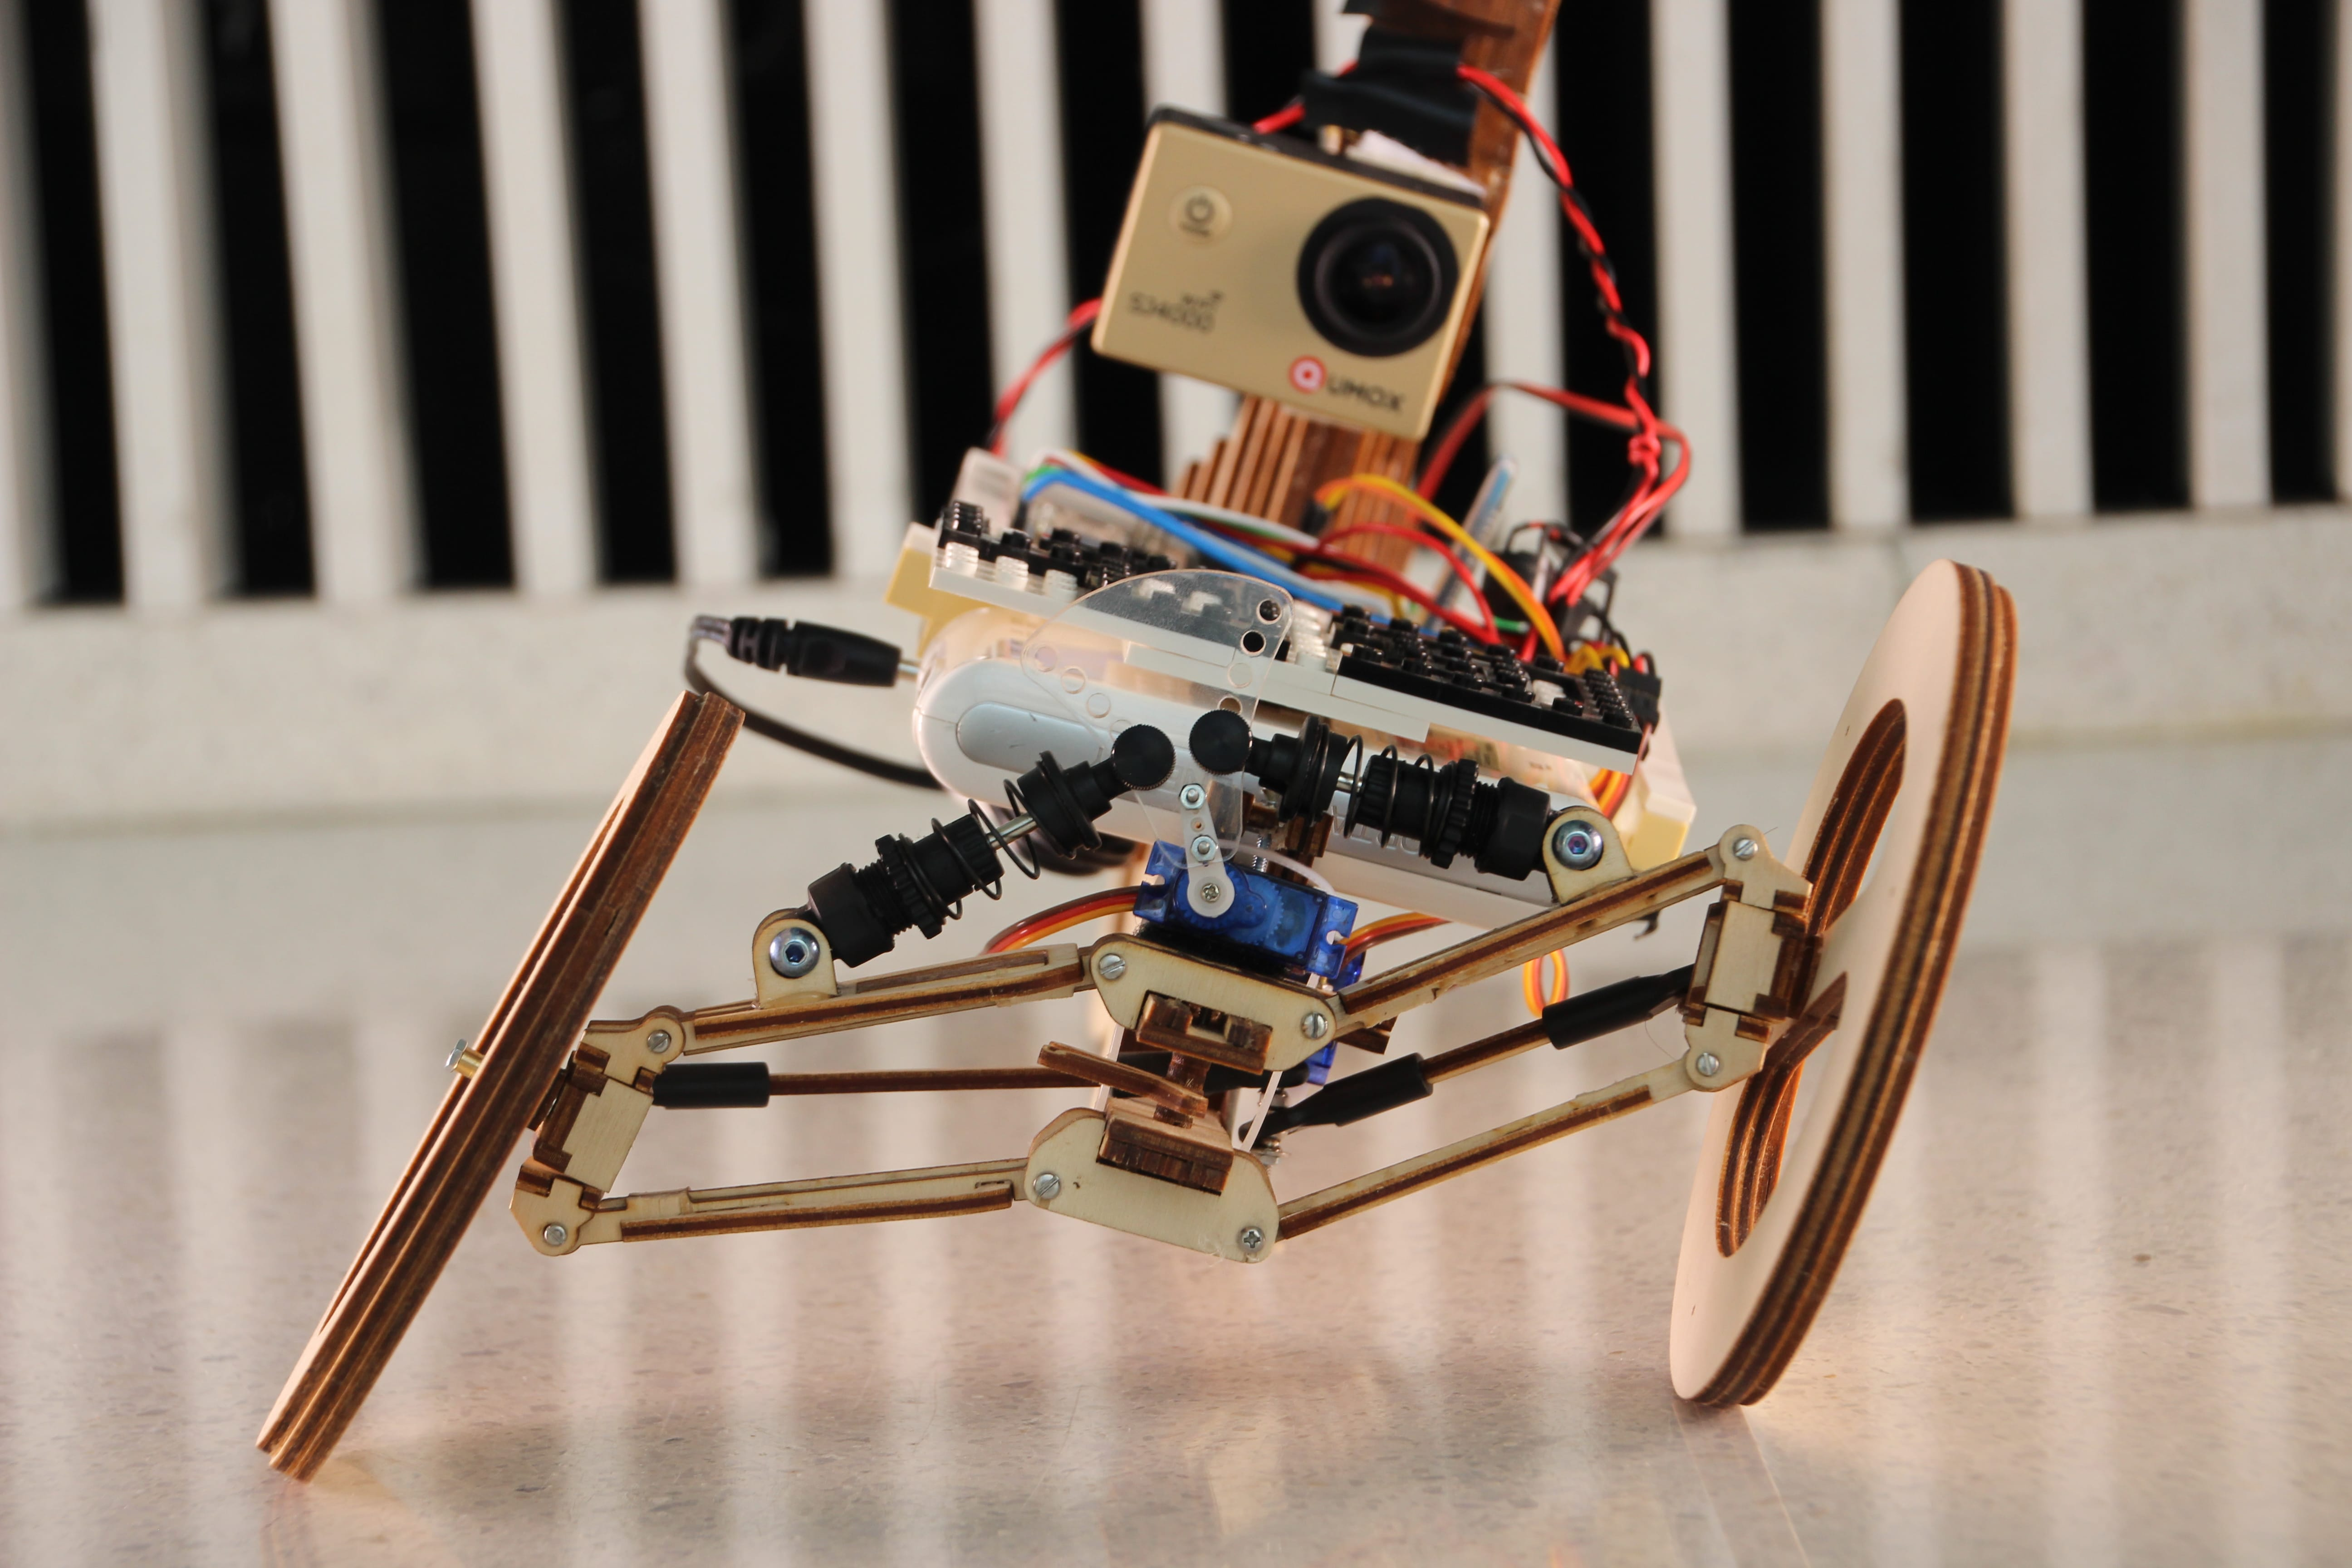
\includegraphics[width=1.0\linewidth]{figs/04/IMG0956}
	\caption{Front view of the miniPEV}
	\label{minipev2}
\end{figure}

\newpage
The value for the angular velocity (yaw rate) $\dot{\psi}$ is obtained from the gyroscope sensor measurement. However, there is no direct information about the longitudinal velocity of the vehicle.  That is why the linear acceleration in the forward direction $a_{x}$ is integrated, thus estimating the velocity $V$.

A strategy in two steps was carried out to filter and integrate the linear acceleration signal. First, a Kalman filter was used and, in second place, a more manual filtering was implemented. In order to validate the integration algorithms, some live tests were made. These test samples were obtained from the Media Lab elevator, going up and down several times.

\newpage
\textbf{Kalman Filter}

A Kalman filter is an optimal estimation algorithm used to estimate states of a system from indirect and uncertain measurements. The most simple Kalman filter has some variables: $x$ for the filtered value, $q$ for the process noise, $r$ for the sensor noise, $p$ for the estimated error and $k$ for the Kalman Gain. 

The filter is applied with each measurement and initialized with the process noise $q$, the sensor noise $r$, the initial estimated error $p$ and the initial value $x=0$. The initial value for $p$ is not very important since it is adjusted during the process. It must be just high enough to narrow down. The filter can be summed up in two simple steps:

\begin{itemize}
\begin{itemize}
	\item Predict
	
	The current state $x_{k}$ is estimated from the previous state $x_{k-1}$ and the estimated error $p$ increases by the inherent process noise $q$.\[x_{k}=x_{k-1}, \quad p=p+q\]
	\item Measurement Update
	
	The kalman gain $k$ balances the relevance of the current observation $z_{k}$ and the previous state $\hat{x}_{k-1}$. It is the ratio of the estimated error $p$ and the noise coming from the sensor $r$. \[k=\frac{p}{p+r}, \quad \hat{x}_{k}=\hat{x}_{k-1}+k(z_{k}-\hat{x}_{k-1})\] When the gain is 0, the current observation has no effect on the updated value, whereas if its value is 1 the previous state does not have an influence.

\end{itemize}
\end{itemize}

After filtering the acceleration $a_x$ with $x_{0}=0 \quad p=1\quad q=0.01\quad r=0.15\quad$, the velocity is integrated with the \textbf{trapezoidal rule of numerical integration}: \[\hat{v}_{k}=\hat{v}_{k-1}+(a_{k}+a_{k-1})\frac{\Delta t}{2}\] The issue with this strategy is the shift of the velocity origin due to the noise in the acceleration and the error in the time interval. These errors accumulate during the ups and downs in the elevator, and incorrectly gives non-zero values of the velocity.

There is an extended Kalman filter that accounts for this shift issue, but is designed to correct the possible shifts in the sensors signals, that is, to fix any possible deviation in the signal coming from the IMU. In this case, we are trying to deal with a numerical integration, not a shift in the signal from the IMU. Therefore, this path is not applicable to this case.

The Kalman filter is perfect for filtering the noise from the accelerometer, but it is not enough to give a good estimation of the velocity when integrating the filtered acceleration. 

\begin{figure}[h!]
	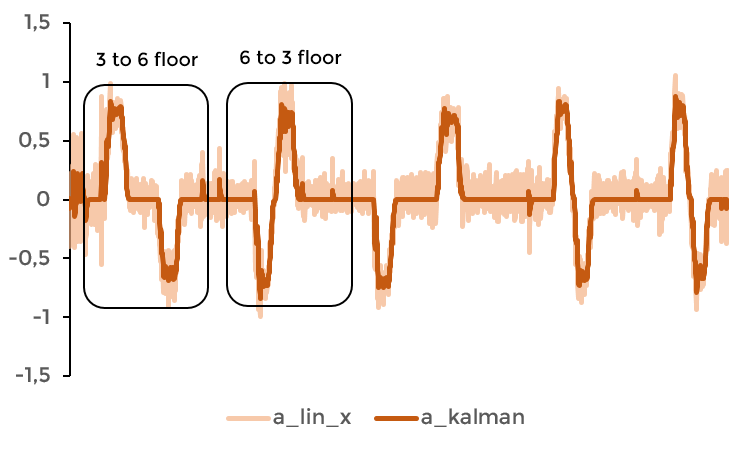
\includegraphics[width=1.0\linewidth]{figs/04/acceleration/1}
	\caption{Kalman filtering to elevator test}
\end{figure}
\begin{figure}[h!]
	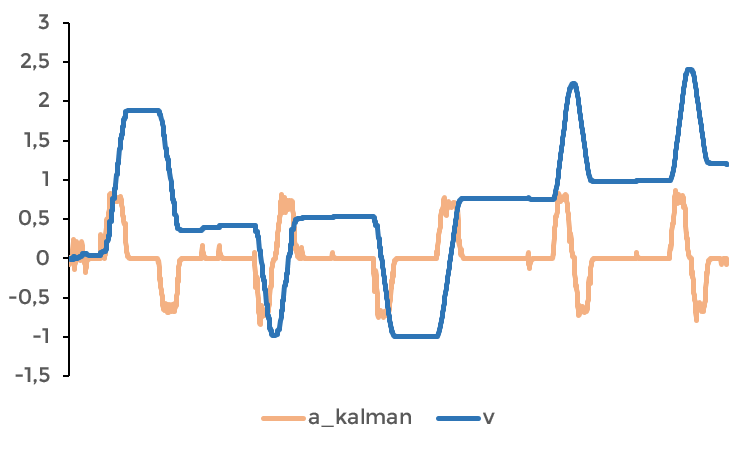
\includegraphics[width=1.0\linewidth]{figs/04/acceleration/2}
	\caption{Elevator velocity estimation with trapezoidal rule}
\end{figure}

\textbf{Integration Shift}

In order to fix the accumulative error in the integration of the acceleration, a very simple algorithm was implemented. This algorithm just corrected the shift by estimating the slope ($m$) of the error during an early sample. 

\begin{itemize}
\begin{itemize}
	\item Trapezoidal
	\[\hat{v}_{k}=\hat{v}_{k-1}+(a_{k}+a_{k-1})\frac{\Delta t}{2}\]

	\item Corrected:
	\[\hat{v}_{k}=\hat{v}_{k-1}+(a_{k}+a_{k-1})\frac{\Delta t}{2}-m\,\Delta t\]
\end{itemize}
\end{itemize}
\newpage

\begin{figure}[h!]
	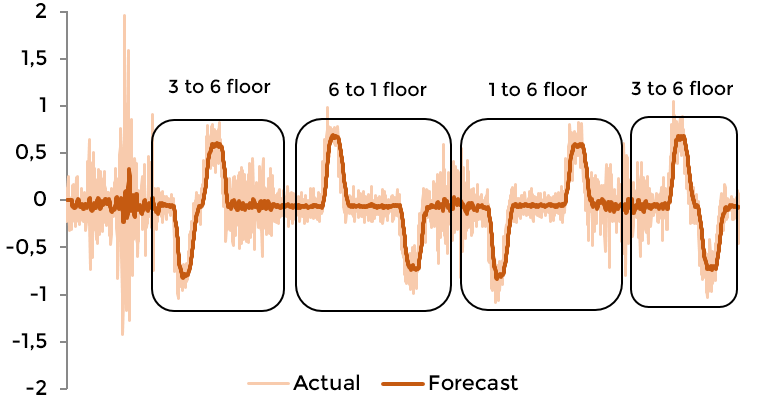
\includegraphics[width=1.0\linewidth]{figs/04/acceleration/3}
	\caption{Sample from the elevator}
\end{figure}
\begin{figure}[h!]
	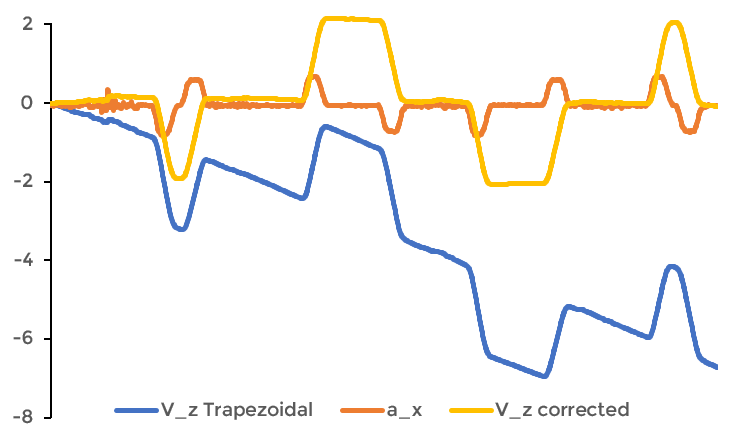
\includegraphics[width=1.0\linewidth]{figs/04/acceleration/4}
	\caption{Acceleration, and integration with trapezoidal rule and a corrected estimation}
\end{figure}

After calibrating this algorithm, a final test was carried out in the elevator, giving good results (Figure \ref{filtered}).

\begin{figure}[h!]
	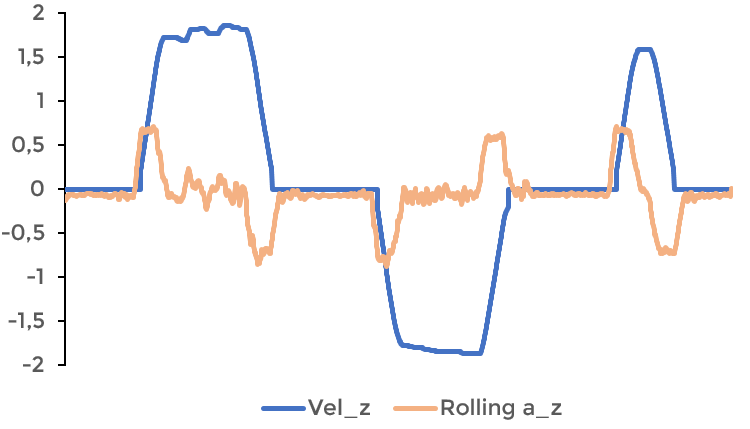
\includegraphics[width=1.0\linewidth]{figs/04/acceleration/6}
	\caption{Final test in the elevator}
	\label{filtered}
\end{figure}


\section{Chapter Conclusions}

The design and fabrication of the miniPEV supposed the first step in this project, and has been really useful for understanding the possible problems that could rise in a tilting vehicle of bigger dimensions. Sometimes looking at a prototype for five minutes is much more productive than thinking about its design and making hundreds of sketches. It also was useful to explain to the Changing Places group and other labmates the ideas that were being developed. 

\begin{marginfigure}
	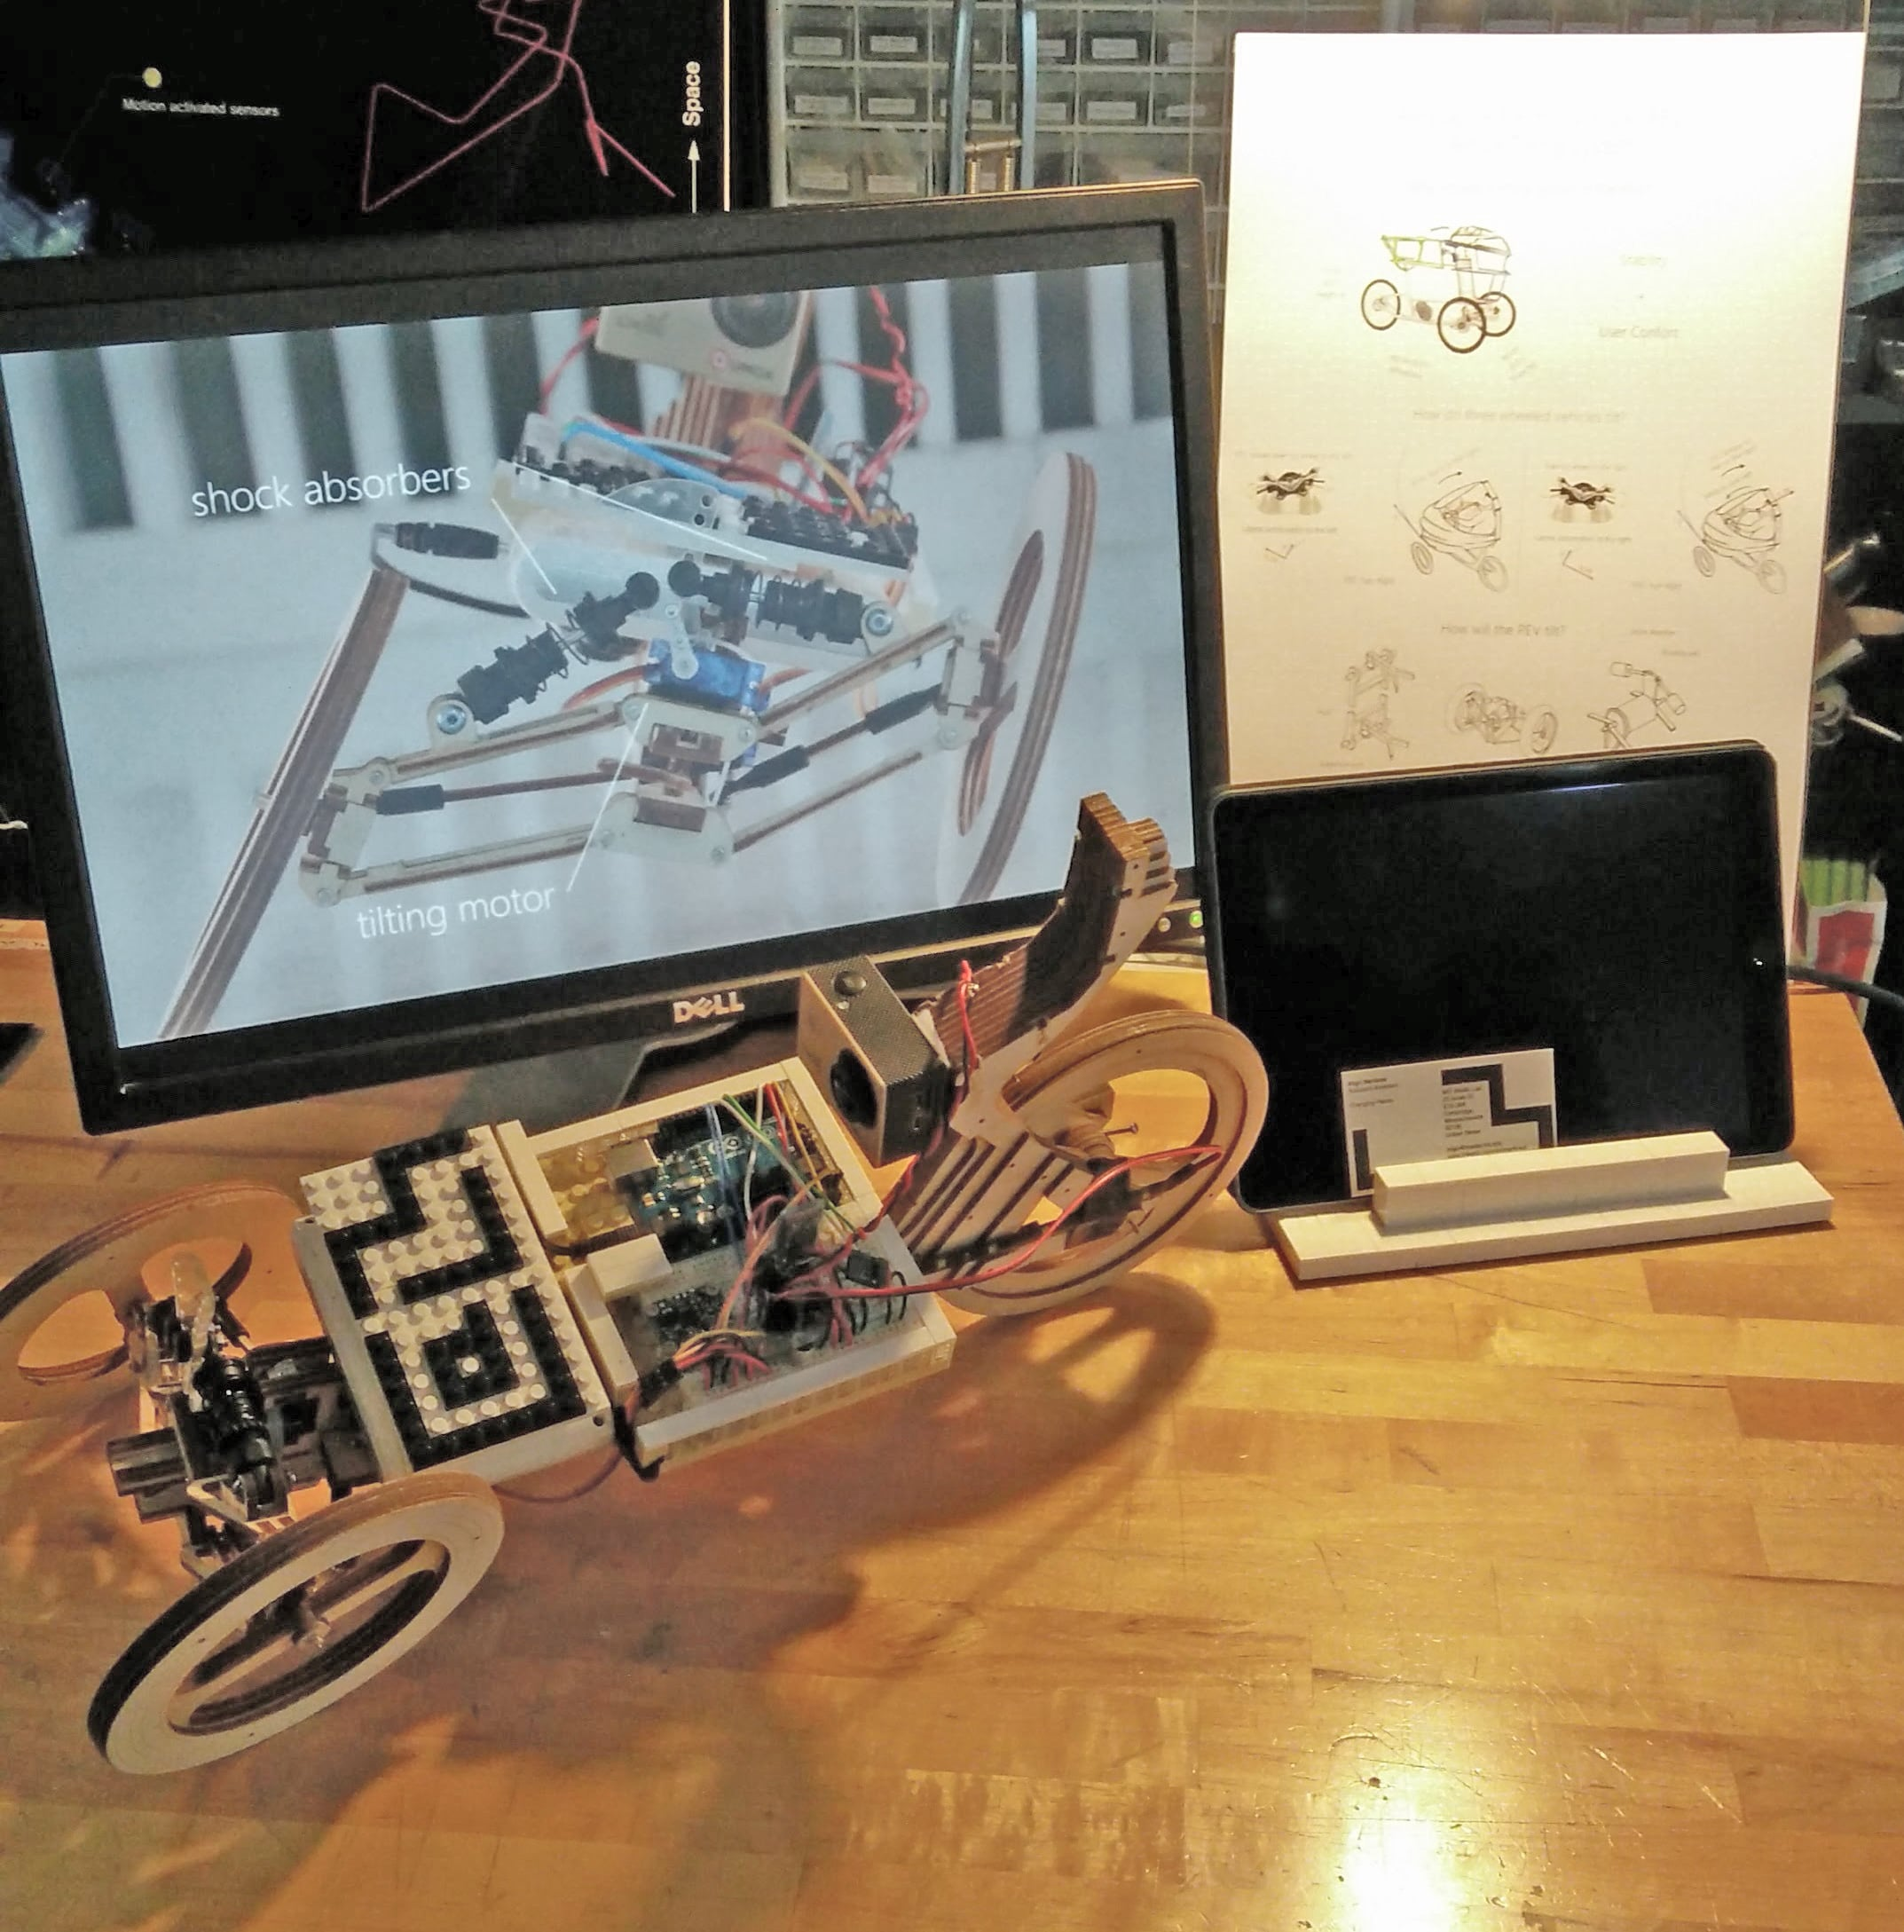
\includegraphics[width=1.0\linewidth]{figs/04/sponsors_fall2}
	\caption{miniPEV stand at the Media Lab Members Event Fall 2016}
\end{marginfigure}

In the technical side, there were some challenges. First, the estimation of the longitudinal speed of the vehicle required several tests and some time going up and down in the Media Lab elevator (which was kind of fun). The results of these test were useful for the integration of other variables in the full scale vehicle.

Regarding the tilting control, the delay between the input from the driver and the action from the motor was evident. This agrees with the studies mentioned previously in the literature review.

Overall, the vehicle satisfactorily performed as expected, and the tilting worked perfectly, even though the motor-actuated glass part was larger than in the initial design. In the next chapter the real scale PEV will be presented.

\begin{figure}[h!]
	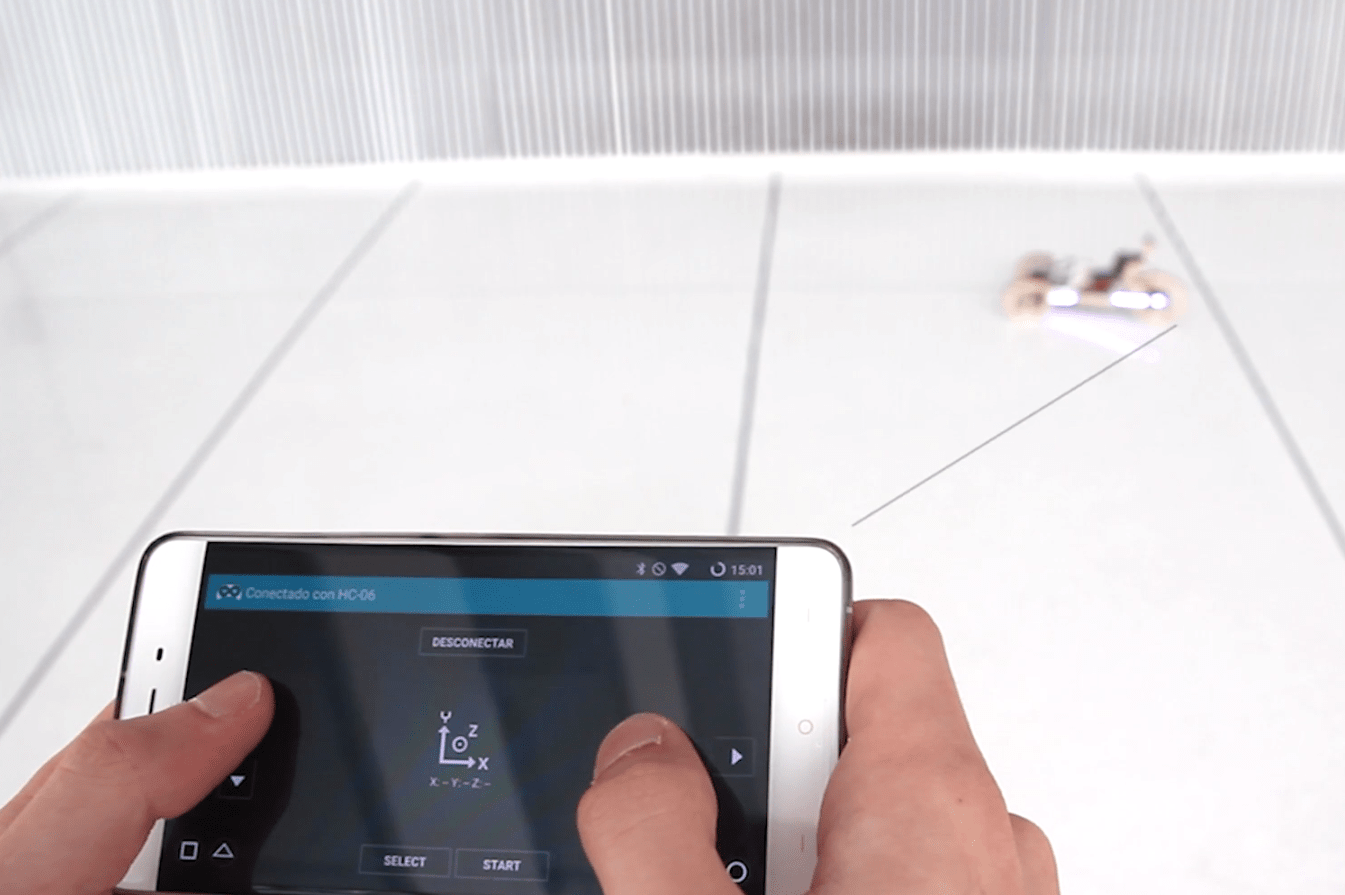
\includegraphics[width=1.0\linewidth]{figs/04/remote}
	\caption{Remote control from the phone to the miniPEV via Bluetooth}
	%\label{filtered}
\end{figure}

